%%%%%%%%%%%%%%%%%%%%%%%%%%%%%%%%%%%%%%%%%%%%%%%%%%%%%%%%%%%%%%%%%%%%%%%%
%% Customizações do abnTeX2 (http://abnTeX2.googlecode.com)           %%
%% para a Universidade de Fortaleza						              %%
%%                                                                    %%
%% This work may be distributed and/or modified under the             %%
%% conditions of the LaTeX Project Public License, either version 1.3 %%
%% of this license or (at your option) any later version.             %%
%% The latest version of this license is in                           %%
%%   http://www.latex-project.org/lppl.txt                            %%
%% and version 1.3 or later is part of all distributions of LaTeX     %%
%% version 2005/12/01 or later.                                       %%
%%                                                                    %%
%% This work has the LPPL maintenance status `maintained'.            %%
%%                                                                    %%
%% The Current Maintainer of this work is Bruno Lopes                 %%
%%                                                                    %%
%% Project available on: https://github.com/bruno-unifor/unifortex2   %%
%%                                                                    %%
%% Further information about abnTeX2                                  %%
%% are available on http://abntex2.googlecode.com/                    %%
%%                                                                    %%
%%%%%%%%%%%%%%%%%%%%%%%%%%%%%%%%%%%%%%%%%%%%%%%%%%%%%%%%%%%%%%%%%%%%%%%%

%%%%%%%%%%%%%%%%%%%%%%%%%%%%%%%%%%%%%%%%%%%%%%%%%%%%%%%%%%%%%%%%%%%%%%%%
%% Customizações do abnTeX2 (http://abnTeX2.googlecode.com)           %%
%% para a Universidade de Fortaleza						              %%
%%                                                                    %%
%% This work may be distributed and/or modified under the             %%
%% conditions of the LaTeX Project Public License, either version 1.3 %%
%% of this license or (at your option) any later version.             %%
%% The latest version of this license is in                           %%
%%   http://www.latex-project.org/lppl.txt                            %%
%% and version 1.3 or later is part of all distributions of LaTeX     %%
%% version 2005/12/01 or later.                                       %%
%%                                                                    %%
%% This work has the LPPL maintenance status `maintained'.            %%
%%                                                                    %%
%% The Current Maintainer of this work is Bruno Lopes                 %%
%%                                                                    %%
%% Project available on: https://github.com/bruno-unifor/unifortex2   %%
%%                                                                    %%
%% Further information about abnTeX2                                  %%
%% are available on http://abntex2.googlecode.com/                    %%
%%                                                                    %%
%%%%%%%%%%%%%%%%%%%%%%%%%%%%%%%%%%%%%%%%%%%%%%%%%%%%%%%%%%%%%%%%%%%%%%%%

\documentclass[
    a4paper,          % Tamanho da folha A4
    12pt,             % Tamanho da fonte 12pt
    chapter=TITLE,    % Todos os capitulos devem ter caixa alta
    section=TITLE,    % Todas as secoes devem ter caixa alta
    oneside,          % Usada para impressao em apenas uma face do papel
    english,          % Hifenizacoes em ingles
    spanish,          % Hifenizacoes em espanhol
    brazil            % Ultimo idioma eh o idioma padrao do documento
]{abntex2}

% Importações de pacotes
\usepackage[brazil]{babel} 
\usepackage[utf8]{inputenc}                         % Acentuação direta
\usepackage[T1]{fontenc}                            % Codificação da fonte em 8 bits
\usepackage{graphicx}                               % Inserir figuras
\usepackage{amsfonts, amssymb, amsmath}             % Fonte e símbolos matemáticos
\usepackage{booktabs}                               % Comandos para tabelas
\usepackage{verbatim}                               % Texto é interpretado como escrito no documento
\usepackage{multirow, array}                        % Múltiplas linhas e colunas em tabelas
\usepackage{indentfirst}                            % Endenta o primeiro parágrafo de cada seção.
\usepackage{listings}                               % Utilizar codigo fonte no documento
\usepackage{xcolor}
\usepackage{microtype}                              % Para melhorias de justificação?
\usepackage[portuguese,ruled,lined]{algorithm2e}    % Escrever algoritmos
\usepackage{algorithmic}                            % Criar Algoritmos
%\usepackage{float}                                  % Utilizado para criação de floats
\usepackage{amsgen}
\usepackage{lipsum}                                 % Usar a simulação de texto Lorem Ipsum
%\usepackage{titlesec}                               % Permite alterar os títulos do documento
\usepackage{tocloft}                                % Permite alterar a formatação do Sumário
\usepackage{etoolbox}                               % Usado para alterar a fonte da Section no Sumário
\usepackage[nogroupskip,nonumberlist,acronym]{glossaries}                % Permite fazer o glossario
\usepackage{caption}                                % Altera o comportamento da tag caption
\usepackage[alf, abnt-emphasize=bf, bibjustif, recuo=0cm, abnt-etal-cite=3, abnt-etal-list=0,abnt-etal-text=it]{abntex2cite}  % Citações padrão ABNT
%\usepackage[bottom]{footmisc}                      % Mantém as notas de rodapé sempre na mesma posição
%\usepackage{times}                                 % Usa a fonte Times
\usepackage{mathptmx}                               % Usa a fonte Times New Roman
%\usepackage{lmodern}                               % Usa a fonte Latin Modern
%\usepackage{subfig}                                % Posicionamento de figuras
%\usepackage{scalefnt}                              % Permite redimensionar tamanho da fonte
%\usepackage{color, colortbl}                       % Comandos de cores
%\usepackage{lscape}                                % Permite páginas em modo "paisagem"
%\usepackage{ae, aecompl}                           % Fontes de alta qualidade
%\usepackage{picinpar}                              % Dispor imagens em parágrafos
%\usepackage{latexsym}                              % Símbolos matemáticos
%\usepackage{upgreek}                               % Fonte letras gregas
\usepackage{appendix}                               % Gerar o apendice no final do documento
\usepackage{paracol}                                % Criar paragrafos sem identacao
\usepackage{lib/unifortex2}		                    % Biblioteca com as normas da Unifor para trabalhos academicos
\usepackage{pdfpages}                               % Incluir pdf no documento
\usepackage{amsmath}                                % Usar equacoes matematicas

% Organiza e gera a lista de abreviaturas, simbolos e glossario
\makeglossaries

% Gera o Indice do documento
\makeindex


%%%%%%%%%%%%%%%%%%%%%%%%%%%%%%%%%%%%%%%%%%%%%%%%%%%%%
%%          Configuracoes do uniforTeX2            %%
%%%%%%%%%%%%%%%%%%%%%%%%%%%%%%%%%%%%%%%%%%%%%%%%%%%%%

% Opcoes disponiveis

\trabalhoacademico{tccgraduacao}
%\trabalhoacademico{tccespecializacao}
%\trabalhoacademico{dissertacao}
%\trabalhoacademico{tese}

% Define se o trabalho eh uma qualificacao
% Coloque 'nao' para versao final do trabalho

%\ehqualificacao{nao}

% Remove as bordas vermelhas e verdes do PDF gerado
% Coloque 'sim' pare remover

\removerbordasdohyperlink{sim}

% Adiciona a cor Azul a todos os hyperlinks

\cordohyperlink{nao}

%%%%%%%%%%%%%%%%%%%%%%%%%%%%%%%%%%%%%%%%%%%%%%%%%%%%%
%%          Informação sobre a IES                 %%
%%%%%%%%%%%%%%%%%%%%%%%%%%%%%%%%%%%%%%%%%%%%%%%%%%%%%

\ies{Universidade de Fortaleza}
\iessigla{UNIFOR}
\centro{Centro de Ciências Tecnológicas}

%%%%%%%%%%%%%%%%%%%%%%%%%%%%%%%%%%%%%%%%%%%%%%%%%%%%%
%%        Informação para TCC de Graduacao         %%
%%%%%%%%%%%%%%%%%%%%%%%%%%%%%%%%%%%%%%%%%%%%%%%%%%%%%

\graduacaoem{Engenharia de Controle e Automação}
\habilitacao{bacharel} % Pode colocar tambem 'licenciada'

%%%%%%%%%%%%%%%%%%%%%%%%%%%%%%%%%%%%%%%%%%%%%%%%%%%%%
%%     Informação para TCC de Especializacao       %%
%%%%%%%%%%%%%%%%%%%%%%%%%%%%%%%%%%%%%%%%%%%%%%%%%%%%%

\especializacaoem{Alfabetização de Crianças}

%%%%%%%%%%%%%%%%%%%%%%%%%%%%%%%%%%%%%%%%%%%%%%%%%%%%%
%%         Informação para Dissertacao             %%
%%%%%%%%%%%%%%%%%%%%%%%%%%%%%%%%%%%%%%%%%%%%%%%%%%%%%

\programamestrado{Programa de Pós-Graduação em Informática Aplicada}
\nomedomestrado{Mestrado Acadêmico em Ciência da Computação}
\mestreem{Ciência da Computação}
\areadeconcentracaomestrado{Ciência da Computação}

%%%%%%%%%%%%%%%%%%%%%%%%%%%%%%%%%%%%%%%%%%%%%%%%%%%%%
%%               Informação para Tese              %%
%%%%%%%%%%%%%%%%%%%%%%%%%%%%%%%%%%%%%%%%%%%%%%%%%%%%%

\programadoutorado{Programa de Pós-Graduação em Informática Aplicada}
\nomedodoutorado{Doutorado em Saúde Coletiva}
\doutorem{Saúde Coletiva}
\areadeconcentracaodoutorado{Saúde Coletiva}

%%%%%%%%%%%%%%%%%%%%%%%%%%%%%%%%%%%%%%%%%%%%%%
%%  Informação relacionadas ao trabalho     %%
%%%%%%%%%%%%%%%%%%%%%%%%%%%%%%%%%%%%%%%%%%%%%%

\autor{Pedro Benevides Cavalcante}
\titulo{Inteligência Artificial aplicada a plataforma robótica Jaguar}
\data{2017}
\local{Fortaleza -- Ceará}

% Exemplo: \dataaprovacao{01 de Janeiro de 2012}
\dataaprovacao{01 de Janeiro de 2017}

%%%%%%%%%%%%%%%%%%%%%%%%%%%%%%%%%%%%%%%%%%%%%
%%     Informação sobre o Orientador       %%
%%%%%%%%%%%%%%%%%%%%%%%%%%%%%%%%%%%%%%%%%%%%%

\orientador{Afonso Henrique Fontes Neto Segundo}
\orientadories{Universidade de Fortaleza - UNIFOR}
\orientadorcentro{Centro de Ciências Tecnológicas - CCT}
\orientadorfeminino{nao} % Coloque 'sim' se for do sexo feminino

%%%%%%%%%%%%%%%%%%%%%%%%%%%%%%%%%%%%%%%%%%%%%
%%      Informação sobre o Co-orientador   %%
%%%%%%%%%%%%%%%%%%%%%%%%%%%%%%%%%%%%%%%%%%%%%

% Deixe o nome do coorientador em branco para remover do documento

\coorientador{}
\coorientadories{Universidade Co-orientador - SIGLA}
\coorientadorcentro{Centro do Co-orientador - SIGLA}
\coorientadorfeminino{nao} % Coloque 'sim' se for do sexo feminino

%%%%%%%%%%%%%%%%%%%%%%%%%%%%%%%%%%%%%%%%%%%%%
%%      Informação sobre a banca           %%
%%%%%%%%%%%%%%%%%%%%%%%%%%%%%%%%%%%%%%%%%%%%%

% Atenção! Deixe o nome do membro da banca para remover da folha de aprovacao

% Exemplo de uso:
% \membrodabancadois{Prof. Dr. Fulano de Tal}
% \membrodabancadoisies{Universidade Estadual do Ceará - UECE}

\membrodabancadois{Membro da Banca Dois}
\membrodabancadoiscentro{Faculdade de Filosofia Dom Aureliano Matos – FAFIDAM}
\membrodabancadoisies{Universidade do Membro da Banca Dois - SIGLA}

\membrodabancatres{Membro da Banca Três}
\membrodabancatrescentro{Centro de Ciências e Tecnologia - CCT}
\membrodabancatresies{Universidade do Membro da Banca Três - SIGLA}

\membrodabancaquatro{Membro da Banca Quatro}
\membrodabancaquatrocentro{Centro de Ciências e Tecnologia - CCT}
\membrodabancaquatroies{Universidade do Membro da Banca Quatro - SIGLA}

\membrodabancacinco{Membro da Banca Cinco}
\membrodabancacincocentro{Teste}
\membrodabancacincoies{Universidade do Membro da Banca Cinco - SIGLA}

\membrodabancaseis{Membro da Banca Seis}
\membrodabancaseiscentro{}
\membrodabancaseisies{Universidade do Membro da Banca Seis - SIGLA}

\begin{document}

	% Elementos pré-textuais
	\imprimircapa
	\imprimirfolhaderosto{}
	\imprimirfichacatalografica{elementos-pre-textuais/ficha-catalografica}
	\imprimirerrata{elementos-pre-textuais/errata}
	\imprimirfolhadeaprovacao
	\imprimirdedicatoria{elementos-pre-textuais/dedicatoria}
	\imprimiragradecimentos{elementos-pre-textuais/agradecimentos}
	\imprimirepigrafe{elementos-pre-textuais/epigrafe}
	\imprimirresumo{elementos-pre-textuais/resumo}
	\imprimirabstract{elementos-pre-textuais/abstract}
	\imprimirlistadeilustracoes
	\imprimirlistadetabelas
	\imprimirlistadequadros
	\imprimirlistadealgoritmos
	\imprimirlistadecodigosfonte
	\imprimirlistadeabreviaturasesiglas
	\imprimirlistadesimbolos{elementos-pre-textuais/lista-de-simbolos}
	\imprimirsumario

	%Elementos textuais
	\textual
	\chapter{Introdução}
\label{cap:introducao}

Cada vez mais à tecnologia avança numa velocidade impressionante. Com esse avanço se tornou possível ter computadores com um grande poder de processamento à um menor custo e ocupando menos espaço. Com isso, algoritmos complexos de inteligência artificial realizam seus cálculos muito mais rápido, além de que, com o tempo, eles foram se tornando cada vez mais robustos \cite{rodrigues2017fundamentos}. 

A \acrlong{IA} (IA) vem evoluindo muito desde à criação do seu conceito, em 1956. Inicialmente, IA era utilizada apenas para à resolução de problemas simples e repetitivos, com aplicação de regras lógicas. Porém, com a chegada da Aprendizagem Profunda (\textit{Deep Learning}) os algoritmos passaram a poder realizar tarefas mais complexas como reconhecimento de fala e classificação de imagens. \cite{goodfellow2016deep}

Outro ramo que vem apresentando um notório crescimento é a industria automobilística. No brasil, ela representa 18,2\% da economia nacional \cite{estadao}, segundo dados de 2011. À adoção de padrões de qualidade, o aumento do nível de exigência dos consumidores e à concorrência do mercado são fatores que impactam diretamente na necessidade de inovação dos veículos produzidos, estimulando o investimento em novas tendências tecnológicas. Entre todas essas tendências, é possível afirmar que à condução autônoma é a mais revolucionária da atualidade. Ela mudará toda à concepção de locomoção veicular que temos. \cite{rodrigues2017fundamentos}

O imenso poder computacional, os complexos algoritmos de inteligência artificial da atualidade e aprendizagem profunda abriu espaço para um sonho antigo ser desenvolvido: os carros autônomos. 
%Com o uso da linguagem \textit{python}, algoritmos de \textit{Deep Learning} e ROS, são adaptados nesse projeto um algoritmo para automatizar a movimentação da Plataforma Robótica Jaguar em duas pistas da Unifor.
Com o uso da linguagem \textit{python}, algoritmos de \textit{Deep Learning} e ROS, é adaptado para a plataforma Robótica Jaguar o algoritmo utilizado no projeto do \textit{Nanodegree} de carros autônomos da Udacity.

\section{Motivação}
\label{sec:motivacao}

Segundo Elon Musk, CEO da \textit{Tesla Motors}, em 2020 já teremos carros autônomos em circulação \cite{elonmusk}, porém o Brasil se encontra em 17º no rank divulgado pelo G1 \cite{brasilutimorank} de países mais aptos à receber à tecnologia, apesar de ter uma excelente aceitação pelos brasileiros, até maior que japoneses. 

As pesquisas divulgadas pelo G1 \cite{brasilutimorank} mostram o quão grande é à dificuldade de aplicação de tecnologia no Brasil. Segundo o rank divulgado pela KPMG \cite{brasilutimorank}, o país ocupa à última posição no rank de política e legislação e o penúltimo no rank de infraestrutura. Isso mostra que, apesar do país ter bastante dificuldades governamentais para a aplicação e desenvolvimento do projeto, não faltam pessoas querendo adquirir essa tecnologia e à corrida para o desenvolvimento desses veículos no país já começou. 

Projetos como o Smart Camaro, IARA, caRINA, e Wally, mostrados na Figura \ref{carrosautonomos} \cite{carroautonomobrasil} já estão em desenvolvimento nas universidades do pais, porém é necessário conhecimentos profundos em ROS (\acrlong{ROS}), programação em C++ e Python, fusão de sensores, visão computacional, programação em GPU (\acrlong{GPU}), além de entendimento sobre \textit{hardware}.

	\begin{figure}[H]
		\centering
		\Caption{\label{carrosautonomos} Smart Camaro, IARA, caRINA, e Wally em ordem}
		\UNIFORfig{}{
			\fbox{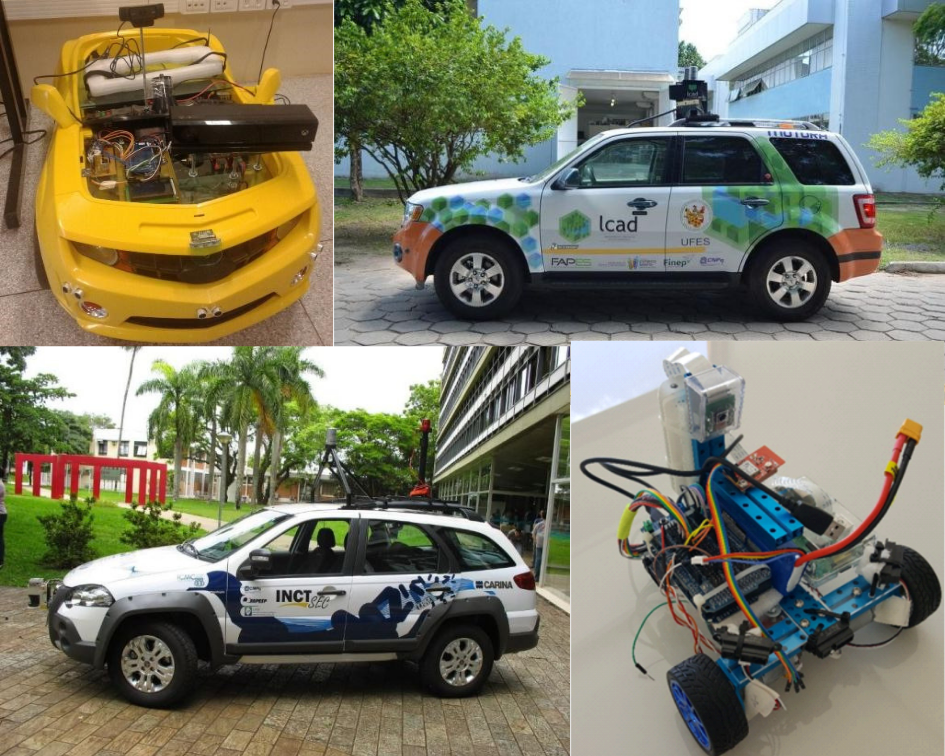
\includegraphics[width=15cm]{fig/carrosAutonomo.png}}
		}{
			\Fonte{\cite{carroautonomobrasil}}
		}	
\end{figure}

Então o maior motivador para o desenvolvimento desse trabalho é iniciar pesquisas de desenvolvimento na área de carros autônomos, pois no Brasil é uma área ainda pouco explorada, porém com um imenso potencial no qual diversas empresas além da \textit{Tesla Motors} \cite{empresasenvolvidascomcarrosautonomos} já iniciaram pesquisa e desenvolvimento na área.

\section{Objetivos}
\label{sec:objetivos}

\subsection{Objetivo Geral}
\label{sec:objetivo-geral}

Adaptar o algoritmo do projeto \textit{Car Behavioral Cloning} para Plataforma Robótica Jaguar utilizando apenas uma câmera, capturar imagens e dados de navegação para criar um modelo da rede neural e testá-lo na pista de atletismo da Unifor e em um circuito na sala L4 da Unifor.

\subsection{Objetivos Específicos}
\label{sec:objetivos-especificos}

%\begin{enumerate}
%\item Instalar o ROS \textit{Kinetic} no Ubuntu de Versão 16.04 LTS, criar o %\textit{Workspace} e instalar todos os pacotes;
%\item Instalação do Python 3.5.2 e bibliotecas para ambas as versões do Python %2.7 e 3.5.2;
%\item Alterar as configurações de rede do computador para conectar à máquina com %o Jaguar;
%\item Obter as imagens e comandos de direção e velocidade do treino nas pistas;
%\item Pilotar o Jaguar em pelo menos duas pistas em diferentes direções;
%\item Treinar o algoritmo para o controle autônomo da Plataforma Robótica Jaguar %com diferentes parâmetros;
%\item Testar os modelos criados nas pistas utilizadas para o treinamento;
%\item Avaliar o desempenho do Jaguar nas diferentes pistas, em diferentes %direções e com diferentes padrões de treinamento e tirar uma conclusão dos %resultados;
%\end{enumerate}





\begin{enumerate}
\item Instalar o ROS em no sistema operacional Ubuntu;
\item Adaptar o algoritmo do projeto \textit{Car Behavioral Cloning} para utilizar somente uma câmera;
\item Desenvolver um programa em python que receba as imagens da câmera Jaguar, os dados de aceleração e angulação do robô e salve tudo em arquivo \textit{.csv}:
\item Criar um modelo para a navegação autônoma que consiga percorrer a pista de atletismo da Unifor e um circuito na sala da L4;
\item Testar os modelos criados nas duas pistas;
\end{enumerate}
	\chapter{Fundamentação Teórica}
\label{cap:fundamentacao-teorica}

\section{Jaguar}
\label{sec:jaguar}

 O Jaguar é uma Plataforma Robótica Móvel pertencente a Universidade de Fortaleza – Unifor projetada para aplicações que exigem manobrabilidade robusta e manobrabilidade do terreno. Ele possui quatro braços articulados que convertem o Jaguar aos mais variados tipos de configurações de navegação, facilitando a movimentação e até escalada em vários tipos de terrenos \cite{jaguar}. 

Esse robô também possui video e áudio integrados de alta resolução, bateria, GPS, giroscópio e bússola, tudo para ser controlado remotamente por uma rede sem fio 802.11N \cite{jaguar}. 
Essas características tornam o Jaguar uma excelente plataforma para o uso de inteligência artificial. Ele é mostrado na figura \ref{Jaguar} e a câmera utilizada utilizada para capturar as imagens para o projeto apontada pela seta vermelha.

\begin{figure}[H]
	\centering
	\Caption{\label{Jaguar} Jaguar}
	\UNIFORfig{}{
		\fbox{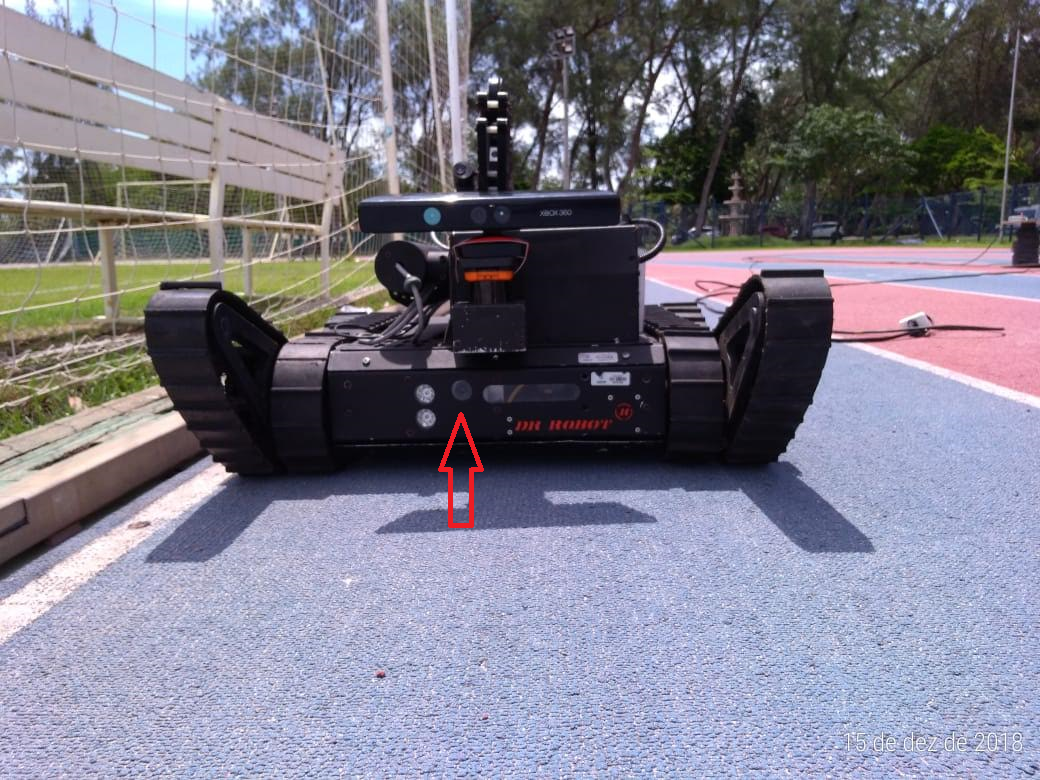
\includegraphics[width=15cm]{figuras/Jaguar.png}}
	}{
		\Fonte{\cite{conv2}}
	}	
\end{figure}

\section{python}
\label{sec:python}

O python é uma linguagem de alto nível orientada a objetos. Ela se tornou tão popular por causa da sua simplicidade, sintaxe clara e concisa e a sua vasta coleção de módulos prontos para o uso \cite{borges2014python}. 

Além de ser utilizada em sistemas operacionais, o python é utilizado em vários softwares para automatização de tarefas (como BrOffice.org, PostgreSQL, Blender, GIMP e Inkscape) \cite{borges2014python}. 

Python é uma linguagem que vem conquistando diversos desenvolvedores e empresas, tal como a Google, a NASA, a IBM, a Embratel e o Serpro. Se comparada a outras linguagens computacionais, provavelmente o python é a que mais oferece bibliotecas para o desenvolvimento de inteligência artificial. Além disso, ela possui uma comunidade de desenvolvedores extremamente ativa, auxiliando o desenvolvimento e aprendizado de novas aplicações nessa linguagem \cite{jonasgranatyr}. 

\section{INTELIGÊNCIA ARTIFICIAL }
\label{sec:INTELIGÊNCIA ARTIFICIAL }

Problemas computacionais sempre foram resolvidos através da programação de
longos códigos, nos quais é especificado cada passo que o computador tem que realizar. Porém, trabalhos que o homem realiza com facilidade pode ser algo bem difícil para ser programado em um computador, como por exemplo o reconhecimento facial, que qualquer acessório ou pequena mudança visual pode dificultar o reconhecimento pelo algoritmo. Essas características, tais como mudança de comportamento, humor e tonalidade da voz são relativamente fáceis de serem percebidas por uma pessoa \cite{lorenafaceli2011inteligencia}. 

%Analise de dados e gráficas são tarefas complexas para serem programadas, principalmente se tiverem que tirar conclusões baseadas nos dados. E, além da complexidade dessas tarefas, é preciso que elas sejam realizadas inúmeras vezes durante um dia. Em alguns casos, o volume de informação é tão grande que se torna impossível de ser analisado por seres humanos \cite{lorenafaceli2011inteligencia}. 
 
Inteligência artificial então é o ramo da computação que procura, por meios computacionais, dar capacidades semelhantes à dos seres humanos para uma máquina, tais como: raciocinar, planejar, resolver problemas, armazenar conhecimento, aprender, perceber e adaptar-se ao meio. \cite{Fernando}.

\section{Aprendizado de Máquina}
\label{sec:aprendizado de máquina}

Estamos em um tempo onde \textit{terabytes} de informações (dados) são criados diariamente. Esses dados podem ser de dois tipos: estruturados (completos sem faltar informação, deixando-o fácil de ser localizado) e não-estruturado (faltando alguma informação nos dados dificultando a sua localização). Se bem trabalhados e analisados, esses dados podem fornecer um grande conhecimento. Cabe então ao algorítimo de Aprendizado de Máquina (ML) trabalhar com esses dados para fazer previsões \cite{pythonmachinelearning}. 

Grandes empresas, como Google, Apple, Amazon, IBM, Microsoft, Facebook e Twitter já usam essa incrível tecnologia. Elas utilizam o \textit{Machine Learning} (Aprendizado de máquina em inglês) para conhecer melhor os seus usuários e fornecer um melhor serviço \cite{pythonmachinelearning}. Um grande exemplo de uso do ML é na analise de sentimentos, onde é possível saber a reação (positiva ou negativa) dos usuários de uma determinada rede social sobre um determinado assunto \cite{sentimentos}.

O algoritmo de \textit{Machine Learning} aprende padrões a partir dos dados entrada juntamente com os seus dados de saída. e pode treinar a máquina para realizar tarefas de forma autônoma. \cite{diferencamachinelearning}.

Em relação ao tipo de aprendizagem, o algoritmo de \textit{Machine Learning} pode ser classificado em três tipos: Aprendizagem Supervisionada (\ref{aprendizadagem supervisionada}), Aprendizagem não supervisionada (\ref{Aprendizagem não supervisionada}) e Aprendizagem por Reforço (\ref{Aprendizagem por Reforço}).

\subsection{Aprendizagem Supervisionada}
\label{aprendizadagem supervisionada}
Nesse tipo de aprendizagem é fornecido para o computador dados rotulados, ou seja, dados de entrada com a sua saída já conhecida. Com isso, é possível prever dados invisíveis ou futuros \cite{pythonmachinelearning}. 
A Aprendizagem Supervisionada pode ser dividida em dois modelos regressão e classificação. No caso da regressão, os dados de entrada são utilizados para criar uma função que gere um valor contínuo. No caso da classificação os dados de entrada são utilizados para mapear os dados de saída em classificações distintas \cite{pythonmachinelearning}. 

\subsection{Aprendizagem não supervisionada}
\label{Aprendizagem não supervisionada}
No caso da Aprendizagem não supervisionada o algoritmo irá trabalhar com dados de entrada nos quais não há praticamente nenhum dado de saída ligado a eles. Ou seja, a máquina terá que gerar uma classificação com os dados de entrada com um determinado padrão entre eles \cite{pythonmachinelearning}. Problemas como esse são normalmente mais complexos principalmente por que não há uma resposta para os dados de teste, tornando assim difícil de avaliar o modelo resultante desse aprendizado.

\subsection{Aprendizagem por Reforço}
\label{Aprendizagem por Reforço}
Através de tentativas e erros, o algoritmo de \textit{Machine Learning} vai procurar uma melhor forma de atuar no ambiente de trabalho para encontrar o sinal de recompensa. Por meio da interação, a máquina procura uma série de ações que levam da melhor maneira possível a recompensa e reduza o erro. Um excelente exemplo dessa aprendizagem é o jogo de xadrez, onde o algoritmo decide, entre uma série de movimentos e o estado do tabuleiro, quais deles vão levar a máquina para vitória e distancia-la da derrota \cite{pythonmachinelearning}.

\section{\textit{Deep Learning}}
\label{deep learning}

Aprendizagem Profunda, em português, é uma forma de aprendizagem de máquina que permite que o computador aprenda através de experiências passadas e compreenda o mundo por uma ideia de hierarquia e conceitos, onde cada nível dessa hierarquia é utilizado para definir outro nível hierárquico. Nesse tipo de aprendizagem não é necessário um operador vistoriando e especificando os conhecimentos necessários para o computador já que ele aprende com experiencias passadas. A hierarquia de conceitos permite que o computador aprenda os conceitos complicados de forma mais simples \cite{goodfellow2016deep}. Então, \textit{Deep learning} (DL) pode ser dito como uma subcategoria do \textit{Machine Learning} que, por meio de algoritmos mais complexos, imita a rede neural do cérebro humano \cite{diferencamachinelearning}.

\textit{Deep Learning} utiliza redes neurais como base do seu algoritmo, porém com muito mais camadas (\textit{Layers}). Foi através dessa subcategoria que tornou-se possível avanços na visão computacional, reconhecimento de fala, processamento de linguagem natural e reconhecimento de áudio.

\section{Redes Neurais Convolucionais}
\label{redes neurais convolucionais}

Rede Neural Convolucional (também conhecida como ConvNet ou CNN) é um tipo de rede neural artificial que pode receber uma imagem de entrada e atribuir importância (com diferentes graus) para vários aspectos ou objetos da imagem e diferenciar um do outro. O pré-processamento de uma rede neural desse tipo é relativamente menor, se comparado aos outros algoritmos de classificação, já que à CNN tem à capacidade de “aprender” o filtro de classificação, enquanto os outros algoritmos necessitam que o filtro seja todo escrito pelo programador\cite{redesneuraisconv,deeplearningbook}.

A primeira proposta de um projeto de rede neural convolucional foi feita em 1988, por Yann LeCun. Seu nome era \textit{LeNet} e era utilizada para o reconhecimento de características numéricas. Ela foi de grande utilidade para impulsionar o campo de pesquisa de \textit{Deep Learning} \cite{redesneuraisconv}.

Os algoritmos de CNN podem dar capacidade ao computador de ver o mundo como um ser humano, conseguindo distinguir diferentes objetos e aspectos da imagem em análise. À figura  \ref{keras_exemple} mostra um excelente exemplo disso, no qual  o algoritmo consegue, com alta taxa de precisão, distinguir os diferentes conteúdos da imagem \cite{conv1,conv2}.

\begin{figure}[H]
	\centering
	\Caption{\label{keras_exemple} Exemplo de reconhecimento de Objetos de uma CNN}
	\UNIFORfig{}{
		\fbox{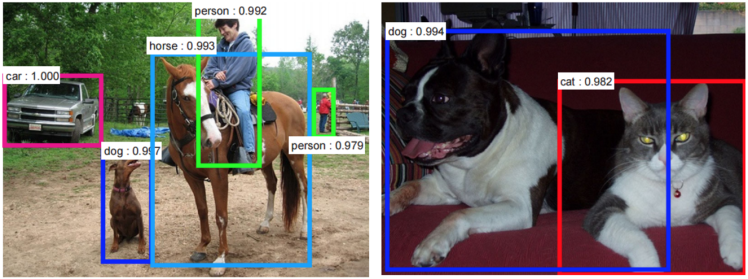
\includegraphics[width=15cm]{fig/keras_exemple.png}}
	}{
		\Fonte{\cite{conv2}}
	}	
\end{figure}

Existem diversas bibliotecas que realizam à implementação de uma Rede Neural Convolucional: \textit{Caffe, MatConvNet, Theano, Torch}. Para esse projeto foi utilizado o \textit{Keras} para o desenvolvimento da Rede Neural, que é uma API de alto nível desenvolvido em python e baseado no \textit{Tensorflow}, biblioteca de aprendizado de máquina  e de código aberto desenvolvida pelo \textit{Google Brain}, em 2015 \cite{redesneuraisconv,keras,tensorflow}.

A arquitetura de uma \textit{ConvNet} é semelhante ao padrão de conectividade dos neurônios dos seres humanos, sendo inspirada na organização do Cortex. \cite{conv1}

 As CNNs possuem diversas comandas, mas há sempre três principais: convolucionais, \textit{pooling} e totalmente conectada. A camada convolucional possui diversos neurônios que tratam de aplicar um filtro em uma determinada parte da imagem. A camada de \textit{pooling} trate de reduzir o tamanho da imagem e fazer a ativação dos pixels mais significativos e a camada totalmente conectada faz a classificação. A figura \ref{exemplo_cnn} mostra uma ilustração de uma CNN.

\begin{figure}[H]
	\centering
	\Caption{\label{exemplo_cnn} Ilustração de uma CNN}
	\UNIFORfig{}{
		\fbox{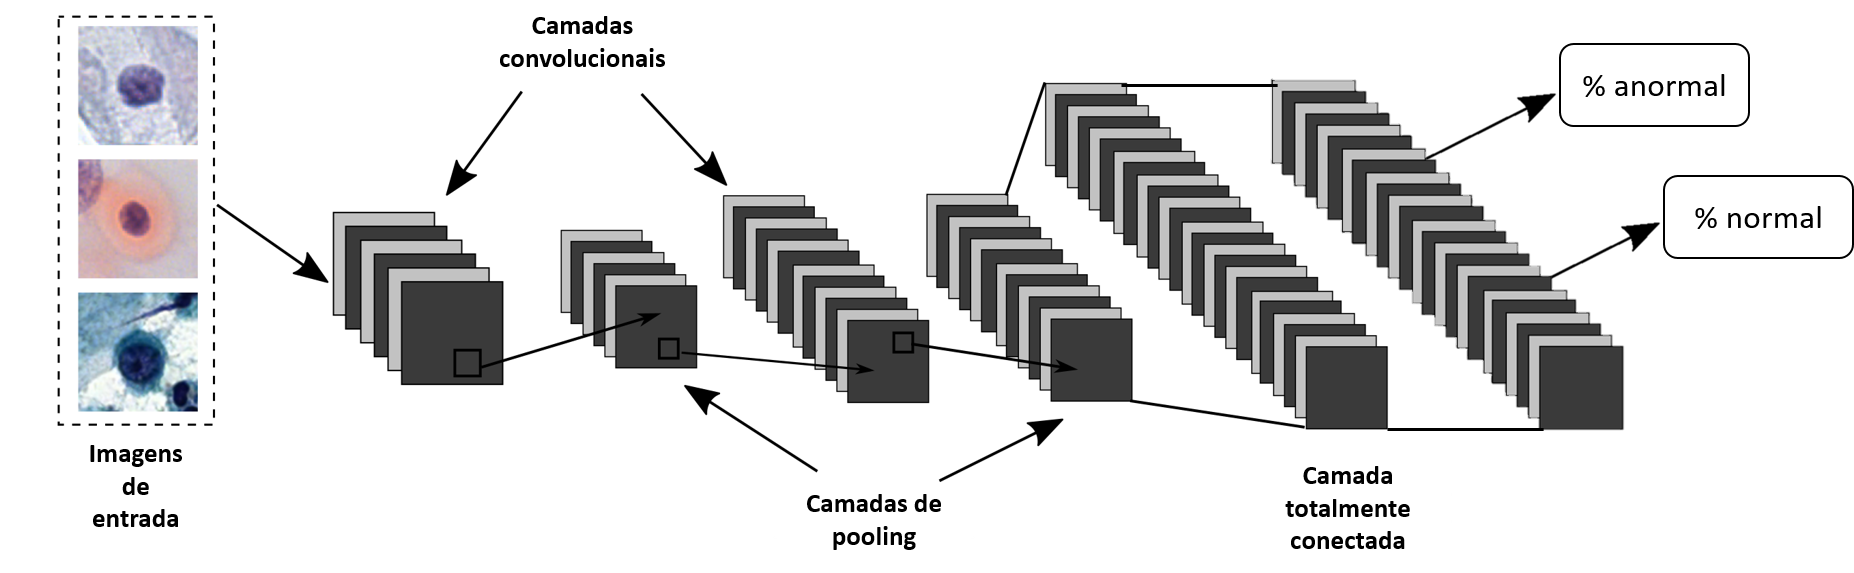
\includegraphics[width=15cm]{fig/exemplo_CNN.png}}
	}{
		\Fonte{\cite{redesneuraisconv}}
	}	
\end{figure}

O volume de entrada que o algoritmo de CNN irá trabalhar é uma imagem. Para entender o funcionamento do algoritmo é preciso primeiramente entender o que é uma imagem na visão computacional\cite{conv2}. 

Basicamente é possível dizer que uma imagem é uma matriz de valores de pixel. Cada valor dessa matriz possui três canais: vermelho, verde e azul, no qual cada um possui um número de 0 a 255 para assim poder formar as cores de cada pixel da imagem. Para imagens em preto e branco existem apenas um canal que também vai de 0 á 255, porém apenas na escala de cinza. 
Com essa visão básica de como é formado uma imagem, é possível compreender como cada uma das camadas da rede neural trabalham em cima dela \textit{resolucao}.

\subsection{Camada Convolucional}

É a primeira camada da CNN. Sua função reduz o tamanho da imagem sem perder suas principais características que são fundamentais para a predição. Para isso, é possível utilizar quantas camadas for necessário \cite{freecodecamp}. É uma camada que consiste em um conjunto de filtros (também conhecidos como \textit{kernels}), que são configurados pela própia CNN enquanto ela vai recebendo dados de entrada, nos quais eles recebem como entrada um arranjo tridimensional, também chamado de volume. Nessa camada nem sempre os neurônios são conectados a todos os neurônios da camada seguinte, como na Rede Neural. Eles se conectam à apenas uma pequena região do mesmo. Conforme a imagem passa por cada camada convolucional ela vai reduzindo assim como o seu filtro \cite{freecodecamp, conv2}.
 
 Uma imagem retirada de um video \textit{Full HD} tem uma resolução de 1920 x 1080 \textit{pixels}, ou seja, 1920 \textit{pixels} na largura e 1080 \textit{pixels} na altura, no qual cada um desses \textit{pixels} há três canais de cores com 256 tonalidades para cada um \cite{resolucao}. Por questões de didáticas, será utilizado um exemplo mais simples de resolução 5 x 5 e apenas um canal de cor com 2 tonalidades.
 \begin{figure}[H]
	\centering
	\Caption{\label{filtro1} Volume de entrada e o Filtro}
	\UNIFORfig{}{
		\fbox{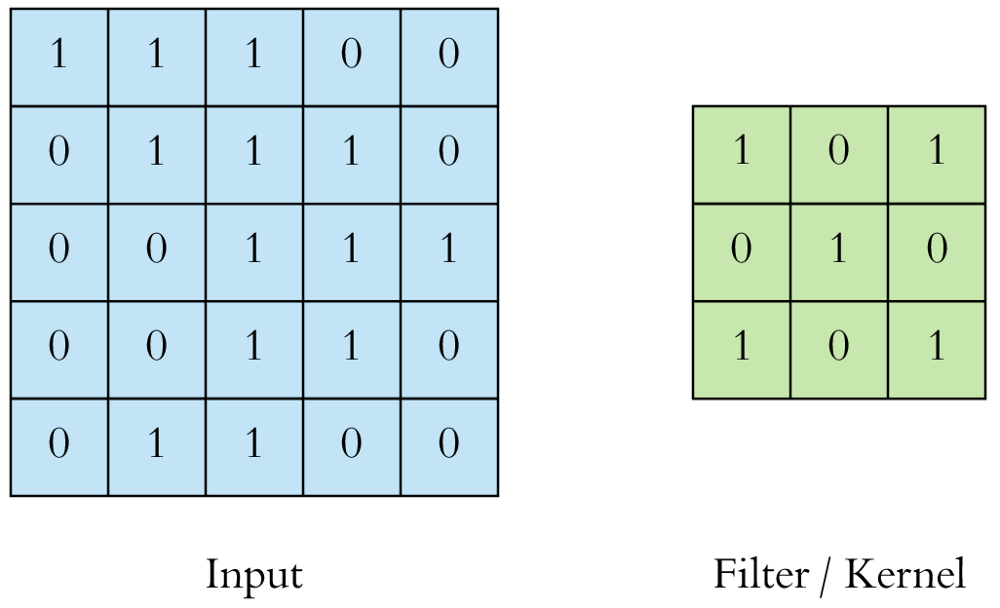
\includegraphics[width=12cm]{fig/filtro3.png}}
	}{
		\Fonte{\ref{freecodecamp}}
	}	
\end{figure}

Na figura \ref{filtro1} temos a Imagem de entrada representada pelo \textit{Input}, onde cada \textit{pixel} é representado por um quadrado da figura e o seu filtro representado por \textit{Filter/Kernel}. O filtro irá passar sobre essa imagem, da esquerda para direta, fazendo o cálculo da matriz da imagem com a matriz do filtro, resultando num mapa de recursos (ou \textit{feature map}), como mostrado na figura \ref{filtro2} \cite{conv2}.

 \begin{figure}[H]
	\centering
	\Caption{\label{filtro2} Mapa de recursos 1}
	\UNIFORfig{}{
		\fbox{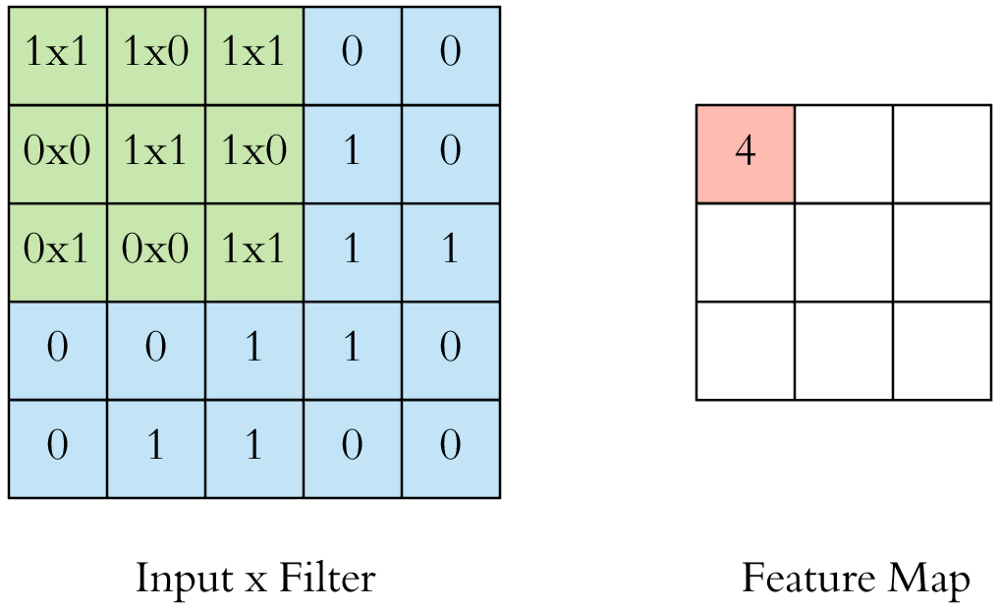
\includegraphics[width=12cm]{fig/filtro2.png}}
	}{
		\Fonte{\cite{freecodecamp}}
	}	
\end{figure}

O filtro percorre, da esquerda para direta e de pixel por pixel, fazendo a multiplicação dos \textit{pixels} da imagem pelos \textit{pixels} do filtro e somando o resultado para criar o mapa de recursos que tem uma linha de pixel a menos em cada um dos seus lados. Esse movimento é repetido linha por linha da imagem de entrada. O resultado Final é mostrado na figura \ref{filtro3} \cite{conv2, freecodecamp}.

 \begin{figure}[H]
	\centering
	\Caption{\label{filtro3} Mapa de recursos 2}
	\UNIFORfig{}{
		\fbox{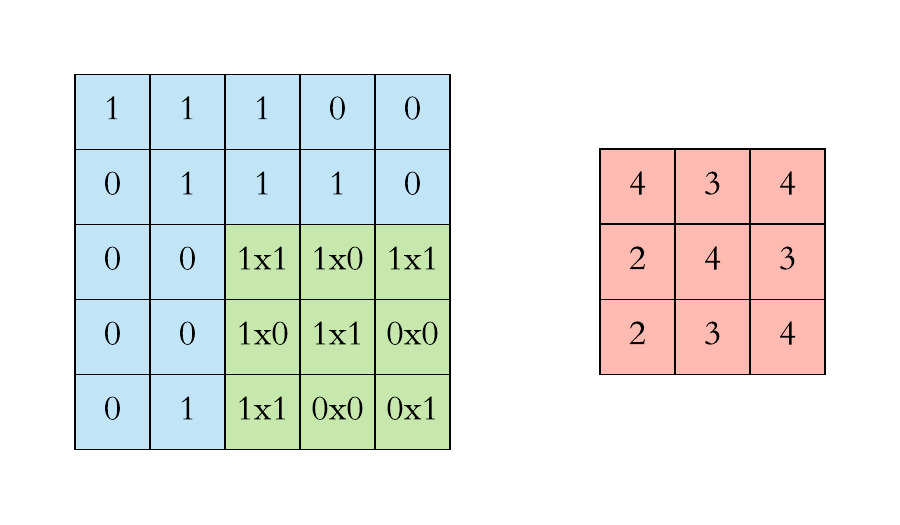
\includegraphics[width=12cm]{fig/filtro4.jpg}}
	}{
		\Fonte{\cite{freecodecamp}}
	}	
\end{figure}

Os filtros podem possuir diferentes valores, gerando assim diferentes efeitos convolucionais. Com isso é possível realizar operações como detecção de borda, nitidez e borrão com apenas uma mudança de valores numéricos da sua matriz. A figura \ref{filtro4} mostra exemplos de algumas operações. Elas são descritas na primeira coluna (identidade, detecção de bordas, aguçamento e borrão, em ordem). Na coluna do meio tem a matriz do filtro e o resultado convolucional na ultima coluna. Os  valores dos filtros são aprendidos pela CNN, mesmo ainda sendo preciso especificar alguns parâmetros pelo programador como número, tamanho, arquitetura do filtro \cite{conv2, aprendizadoDeMaquinaDivertido}.

\begin{figure}[H]
	\centering
	\Caption{\label{filtro4} Diferentes tipos de Filtros}
	\UNIFORfig{}{
		\fbox{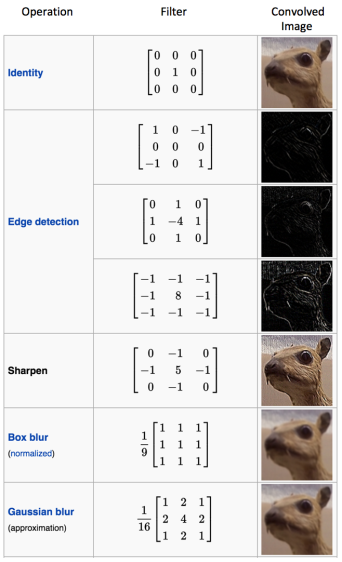
\includegraphics[width=10cm]{fig/tiposdefiltros.png}}
	}{
		\Fonte{\cite{conv2}}
	}	
\end{figure}

O resultado final da convolução, o \textit{feature map} é controlado por três parâmetros:
\begin{description}
    \item[Profundidade:] é o número de filtros usado para a convolução.
    \item[\textit{Stride:}] é o número de \textit{pixel} que o filtro vai percorrer por vez. Por exemplo: se o \textit{Stride} for igual a 1, o filtro vai percorrer apenas 1 pixel por vez.
    \item[\textit{Zero-padding:}] em alguns casos é preciso preencher a borda da matriz de de entrada (a imagem) com zeros para poder controlar o tamanho do mapa de características. 
\end{description}

Ao final de cada operação de convolução também é comum utilizar uma função de não-linearidade, a ReLU. Sua função é substituir todos os \textit{pixels} negativos por zero do mapa de recursos. Então, a Unidade Linear retificadora (ReLU) introduz a não linearidade no resultado final já que a maioria dos dados de entrada reais são não lineares \cite{conv2}.
A Figura \ref{filtro6} mostra um excelente exemplo da aplicação dessa função, onde a imagem da direita é o resultado depois da aplicação do filtro.

\begin{figure}[H]
	\centering
	\Caption{\label{filtro6} Aplicação do Filtro ReLU}
	\UNIFORfig{}{
		\fbox{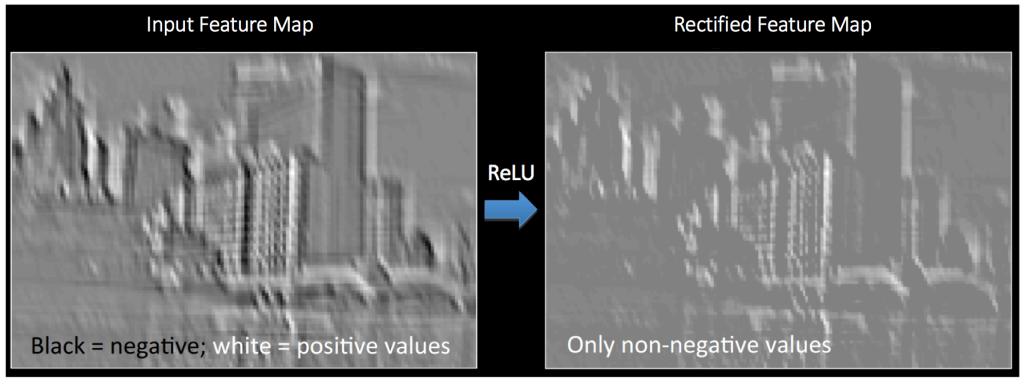
\includegraphics[width=16cm]{fig/relu.png}}
	}{
		\Fonte{\cite{conv2}}
	}	
\end{figure}

Para esse projeto foi utilizado a função de ativação ELU (Unidade Linear Exponencial, ou ingles, \textit{Exponential Linear Unit}). Ela converge mais rapidamente para o zero e possui resultados mais precisos.

Em relação ao ReLU, ela possui uma constante extra positiva, chamada de alfa. Ela também difere do ReLu pela sua suavisão que é mais lente e bem menos acentuada. Podemos ver isso no gráfico da figura \ref{elurelu} \cite{elu}.

\begin{figure}[H]
	\centering
	\Caption{\label{elurelu} Função Elu x ReLU}
	\UNIFORfig{}{
		\fbox{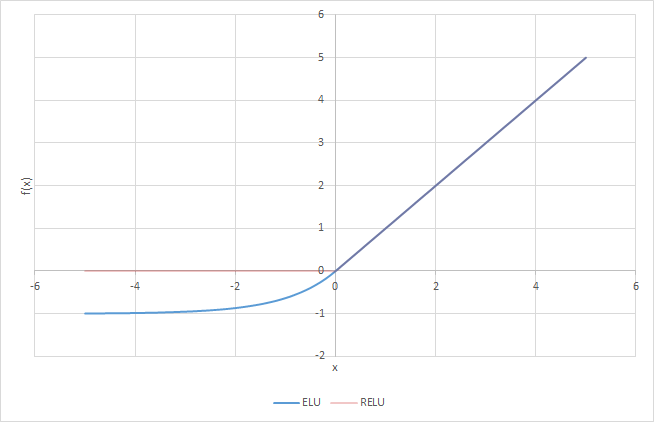
\includegraphics[width=15cm]{fig/elurelu.png}}
	}{
		\Fonte{\cite{elu}}
	}	
\end{figure}

\subsection{Camada de \textit{Pooling}}

A função da camada de \textit{pooling} (também chamada de subamostragem ou \textit{downsampling}) é reduzir a dimensão do mapa de recursos mantendo as informações mais importantes. Podemos ter a soma, a média ou \textit{Max Pooling}, que é a mais popular e também utilizada nesse trabalho. Essa ultima funciona definindo uma janela de \textit{pixels} (por exemplo, uma janela 2x2 onde ela "visualiza" apenas 4 \textit{pixels} do mapa de amostragem) e seleciona o maior deles para montar outro mapa de recursos, como é mostrado na figura \ref{maxpool}. Essa função se aplica por toda a imagem \cite{freecodecamp}.

\begin{figure}[H]
	\centering
	\Caption{\label{maxpool} Aplicação do \textit{Pooling}}
	\UNIFORfig{}{
		\fbox{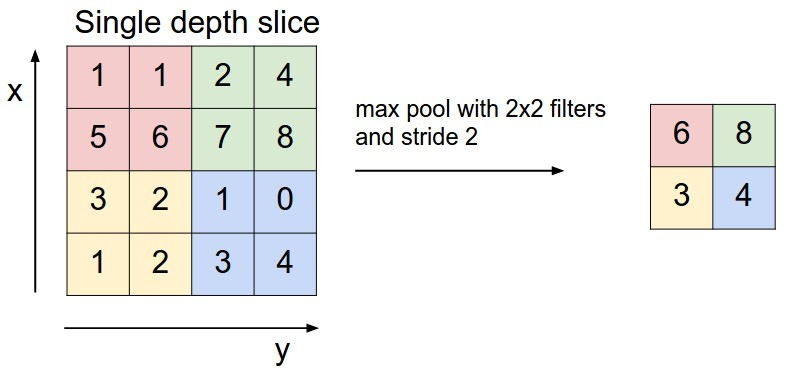
\includegraphics[width=15cm]{fig/maxpool.jpg}}
	}{
		\Fonte{\cite{CS231n}}
	}	
\end{figure}

O resultado da aplicação desse camada é mostrado na figura \ref{pool} (lembrando que já foi aplicado a convolução e ativador ReLU na imagem).

\begin{figure}[H]
	\centering
	\Caption{\label{pool} Exemplo de \textit{Pooling}}
	\UNIFORfig{}{
		\fbox{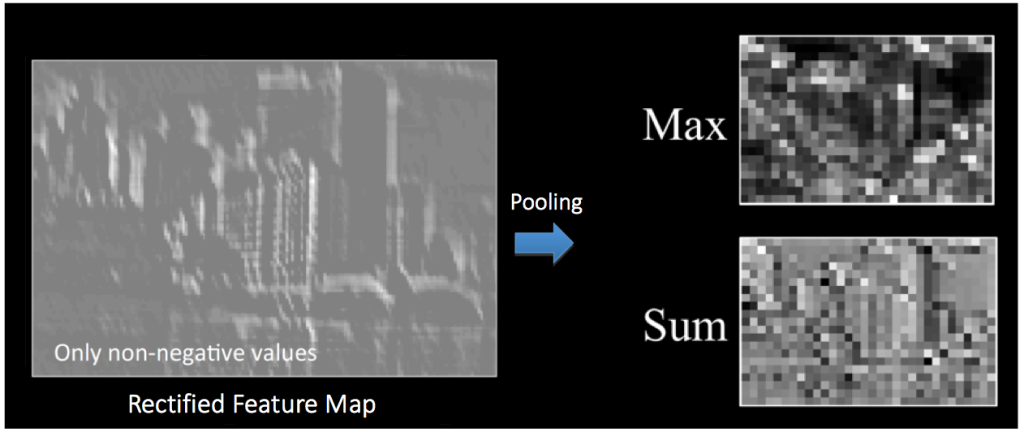
\includegraphics[width=15cm]{fig/pool.png}}
	}{
		\Fonte{\cite{conv2}}
	}	
\end{figure}

\subsection{Camada \textit{Fully Connected}}

Camada totalmente conectada, em português, é uma camada onde todos os neurônios da camada anterior estão totalmente conectados a todos os neurônios da camada posterior. Seu objetivo é classificar as imagens de entrada nos vários grupos determinados pelo \textit{dataset}. Essa é etapa final da predição, onde ela irá retornar um valor para o usuário entre 0 (0\% de probabilidade) e 1 (100\% de probabilidade) referente a cada um dos \textit{datasets}. A figura \ref{exemploCNN} mostra, na sua extremidade direita, o percentual de probabilidade de ser cada um dos \textit{datasets} inseridos. Pode-se observar que o \textit{boat} (barco) tem a maior probabilidade, sendo 0,94.\cite{conv2, aprendizadoDeMaquinaDivertido}. 
Lembrando que esses são as camadas básicos de uma CNN, mas não necessariamente elas precisam sempre seguir essa Ordem. Na figura \ref{exemploCNN}, por exemplo, há duas camadas Convolucionais com ReLU e \textit{Pooling} para no final haver duas camadas totalmente conectadas \cite{conv2}.

\begin{figure}[H]
	\centering
	\Caption{\label{exemploCNN} Exemplo de Rede Neural Convolucional}
	\UNIFORfig{}{
		\fbox{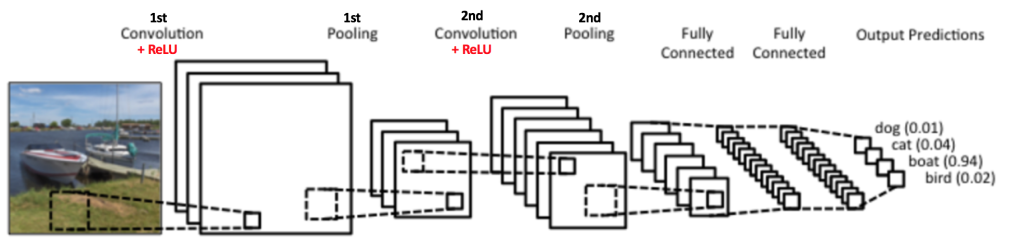
\includegraphics[width=16cm]{fig/exemploCNN.png}}
	}{
		\Fonte{\cite{conv2}}
	}	
\end{figure}
	\chapter{Trabalhos Relacionados}
\label{cap:trabalhos-relacionados}

\section{\textit{End-to-End Deep Learning for Self-Driving Cars}}

Nesse projeto é utilizado Redes Neurais Convolucionais para fazer uma análise profunda das imagens capturadas pela câmera frontal do carro autônomo e gerar os comandos de direção para o veículo. Com esse sistema o computador aprende a pilotar o carro com apenas a análise do treinamento feito por humanos. Diferentemente de outros carros autônomos, o projeto da Nvidia não decompõe a imagem de forma explícita, como por exemplo, procurar o contorno da estrada na imagem. Ele trabalha a imagem como um todo, juntamente com os valores de angulação e aceleração. \cite{nvidiabojarski2016end}

O projeto do jaguar é baseado no algoritmo da Nvidia, porém o computador não tem o mesmo poder de processamento do Jaguar e nem fica ligado diretamente nele, sendo necessário conectar à plataforma através de uma rede wireless. Esse tipo de conexão juntamente com o fraco poder computacional fazem com que o delay seja grande na análise e resposta da imagem do Jaguar.

\section{\textit{Open Source Self-Driving Car}}

Esse projeto é um dos vários cursos pagos oferecidos pela Udacity que, com parceria de grandes empresas como Google, Amazon e Facebook, tem como intuito oferecer um conhecimento que está em alta demanda no mercado de trabalho. No caso do Projeto \textit{Open Source Self-Driving Car} a Udacity oferece um curso no qual o aluno desenvolve o algoritmo de carro autônomo com redes neurais e pode treinar e testar o algoritmo no simulador desenvolvido pela empresa. \cite{self-drivingcar} 

O projeto do Jaguar utiliza um algoritmo parecido com o do projeto do \textit{Self-Driving Car}, porém ele foi testado em um ambiente real com um veículo real e apenas uma simples câmera ao invés de três, como é utilizado no Source Self-Driving Car. Isso tornou o cálculo da rede neural um pouco mais complexo, porém ainda sim ele conseguiu andar de forma autônoma.

\section{\textit{AutoWare}}

O \textit{autoware} é o primeiro \textit{software} de código aberto para carros autônomos baseado em \textit{ROS}. Ele fornece alguns recursos, mas não se limita à somente eles: localização obtida por mapas 3D e algoritmos \textit{SLAM} em combinação com sensores GNSS e IMU, detecção utiliza câmeras e LiDARs com algoritmos de fusão de sensores e redes neurais profundas. Sua predição e planejamento são baseados em robótica probabilística e sistemas baseados em regras, no qual também é utilizado redes neurais profundas. A saída do \textit{Autoware} para o veículo é uma junção de velocidade e ângulo de direção. Esse é a parte do Controle do software, onde os algoritmos PID e MPC são frequentemente adotados. \cite{autoware}

O algoritmo do presente trabalho se limita a trabalhar somente com os dados obtidos da câmera do Jaguar. Através disso é possível gerar os dados de velocidade e angulação da direção para a plataforma Jaguar. Para pistas mais simples não se mostrou necessidade de algo mais complexo.

\section{\textit{Self Driving (Toy) Ferrari}}
\label{Self_Driving_(Toy)_Ferrari}

Esse projeto feito pelo Ryan Zotti tem como intuito fazer um carrinho de brinquedo com um \textit{raspberry Pi} dirigir de forma autônoma utilizando um sensor de distância ultrassônico, uma câmera e um algoritmo de inteligência artificial. Para isso, é preciso primeiro treinar o algoritmo com os dados adquiridos do controle remoto, câmera e sensor de distância. Depois de treinado e criado os modelos é possível colocar o carrinho para andar de forma autônoma. \cite{selfdrivingcartoy}

Esse projeto usa um algoritmo muito parecido com o do Jaguar, porém esse algoritmo trabalha fora do Jaguar, enquanto no projeto do Ryan o algoritmo trabalha dentro do microcontrolador, o que pode exigir um poder de processamento muito maior, porém um \textit{delay} de resposta menor devido a ausência da rede wireless, se comparado ao projeto Jaguar.

\section{NAVEGAÇÃO SEGURA DE UM CARRO AUTÔNOMO UTILIZANDO CAMPOS VETORIAIS E O MÉTODO DA JANELA DINÂMICA}
\label{NAVEGAÇÃO_SEGURA}

Esse trabalho apresenta uma proposta de um modelo de carro autônomo que utiliza planejamento de movimentos por meio de campos vetoriais de velocidade juntamente com o método da janela dinâmica para desviar de obstáculos. Para isso, foi utilizado o carro autônomo que está em desenvolvimento na Universidade Federal de Minas Gerais, o CADU, que utiliza uma câmera estéreo \textit{Bumblebee2} e dois computadores portáteis. Esse projeto foi capaz de circular por um campo vetorial elipsoidal com obstáculo de maneira satisfatória. \cite{marcatto2014desenvolvimento}

Em relação ao Jaguar, os dois projetos têm o mesmo intuito: fazer um veículo autônomo. Porém, além de ser utilizado veículos diferentes, o algoritmo do CADU utiliza campos vetoriais e janela dinâmica enquanto o Jaguar utiliza rede neural convolucional para analisar à sua trajetória de navegação.

\begin{comment}
\Gls{ambiguidade}
\Gls{braile}
\Gls{coerencia}
\Gls{dialetos}
\Gls{elipse}
\Gls{locucao-adjetiva}
\Gls{modificadores}
\Gls{paronimos}
\Gls{sintese}
\Gls{borboleta}
\end{comment}
	\chapter{Metodologia}
\label{chap:metodologia}

Para o desenvolvimento desse projeto, foi utilizado o ROS\textit{ Kinetic}, considerado uma das versões mais estáveis ROS. Ele é compatível apenas com o Ubuntu 16.04, tornando necessário a instalação do mesmo em \textit{dual boot}, mantendo o sistema operacional \textit{Windows} como segunda opção de \textit{boot}. Para isso, o tutorial utilizado para instalar o \textit{Ubuntu} em \textit{dual boot} no computador foi retirado do site \textit{Lcomlinux} \cite{ubuntu}. A Figura\ref{instacaoubuntu} mostra a página inicial de instalação do Ubuntu.

	\begin{figure}[H]
		\centering
		\Caption{{\label{instacaoubuntu}}Página inicial da instalação do Ubuntu}
		\UNIFORfig{}{
			\fbox{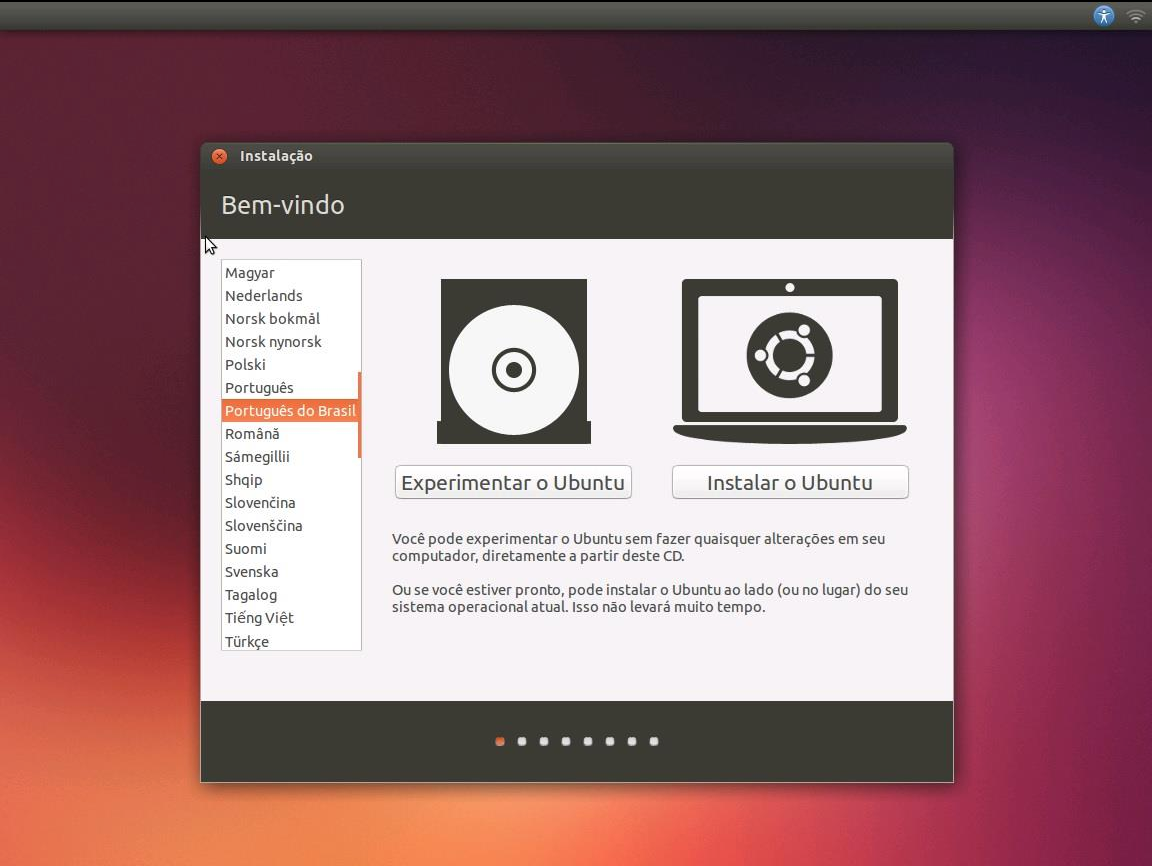
\includegraphics[width=14cm]{figuras/instalacaoubuntu.png}}
		}{
			\Fonte{Elaborado pelo autor}		}	
	\end{figure}
	
Após instalado o sistema, é preciso instalar o ROS e o \textit{python} 3.5 juntamente com os seus respectivos pacotes e biblioteca. O tutorial seguido para instalação do ROS foi retirado do própio site do Ros \cite{rosInstalacao}. Após a sua instalação e criação do seu \textit{Workspace} é preciso instalar os pacotes do Jaguar. Para isso, copie e cole a pasta \textit{DrRobotMotionSensorDriver-master} dentro da pasta src do \textit{Workspace} criada e novamente, no terminal aberto dentro do mesmo \textit{Workspace}, execute o comando catkin\_make. Faça a mesma coisa para a pasta \textit{drrobotV2\_player\-master}.

Caso não funcione, delete a pasta \textit{DrRobotMotionSensorDriver\-master}, mostrada na Figura\ref{arquivosROS} deixando somente o \textit{drrobotV2\_player\-master}, e copie os arquivos da pasta \textit{Drivers Ros/WorkSpace} e substitua os arquivos da sua pasta \textit{Devel} pelos arquivos da pasta fornecida e faça novamente o comando \textit{catkin\_make}. Antes de dar continuidade em qualquer comando no terminal para o ROS, execute o comando \textit{“source ...devel/setup.bash”} (substitua os três pontos pelo caminho do diretório do \textit{Workspace} do \textit{Ros}) depois faça o comando anterior. Normalmente é preciso executar o comando \textit{“source ...devel/setup.bash”} sempre que for executar algum \textit{node} do Jaguar. Esse comando não pode ser adicionado a inicialização do terminal pois ele é incompatível com a versão 3.5 do \textit{python}, tornando impossível a execução de programas \textit{python} dessa versão.

	\begin{figure}[H]
		\centering
		\Caption{\label{arquivosROS}Arquivos do \textit{Workspace} do ROS}
		\UNIFORfig{}{
			\fbox{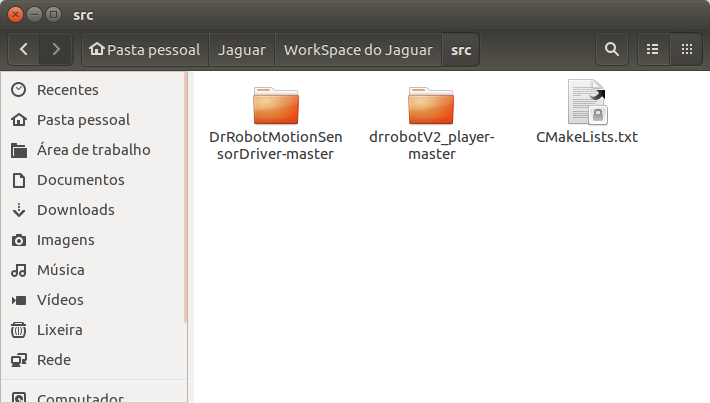
\includegraphics[width=14cm]{figuras/002.png}}
		}{
			\Fonte{Elaborado pelo autor}
		}	
	\end{figure}
	
Após feito a instalação do \textit{ROS} com os pacotes do Jaguar, é preciso instalar o \textit{python} 3.5 e suas bibliotecas para execução do programa. Para instalar o \textit{python} é muito simples: basta apenas executar os comandos abaixo. Eles instalam o \textit{python} 3.5 juntamente com o instalador de pacotes \textit{pip} de versão 2.7 e 3.5.
\begin{lstlisting}
sudo apt-get update
sudo apt-get install python3.5
sudo apt-get install python-pip 
sudo apt-get install python3-pip
\end{lstlisting}
Após a execução dos comandos o computador já deve estar com o \textit{python} e o \textit{pip} pronto para execução. Agora é preciso instalar as bibliotecas. Para o \textit{python} de versão 2.7, execute o seguinte comando no terminal dentro da pasta do projeto: 
\begin{lstlisting}
sudo pip install -r requerimentos2.7.txt
\end{lstlisting}
Para o \textit{python} de versão 3.5, execute o comando:
\begin{lstlisting}
sudo pip3 install -r requerimentos3.5.txt
\end{lstlisting}
Atualize o Ubuntu:
\begin{lstlisting}
sudo apt-get update
\end{lstlisting}
Para testar se todos os comandos foram executados corretamente, a sugestão é executar os arquivos \textit{savefile.py} e \textit{model.py} e verificar quais bibliotecas estão em falta. Para isso, abra o terminal dentro da pasta que se encontra esses dois arquivos e execute os seguintes comandos:
\begin{lstlisting}
Python3.5 savefile.py
\end{lstlisting}
Esse comando irá executar o arquivo \textit{savefile.py}. Se ele não executar, verifique quais bibliotecas estão em falta na janela do terminal. Faça a mesma coisa para o \textit{model.py}, executando o comando:
\begin{lstlisting}
Python model.py
\end{lstlisting}
Com todas as bibliotecas do \textit{python} funcionando, já é possível conectar o computador ao Jaguar. Use a senha 12345678 para conectar à rede “Jaguar”, mas antes modifique as configurações de IPv4 para os seguinte parâmetro:
\begin{lstlisting}
ip: 192.168.0.128
mascara de rede: 255.255.255.0
\end{lstlisting}
Após essa modificação é possível observar que o dispositivo já consegue conectar-se ao jaguar. 

\section{Ligando o ROS}
Para ligar o ROS siga os seguinte passos:

Abra o Terminal (Ctrl + Alt + T) e digite o comando:
\begin{lstlisting}
roscore
\end{lstlisting}
Esse comando irá executar o ROS ná máquina.

Abra outro terminal e execute:
\begin{lstlisting}
source (diretório do workspace)/devel/setup.bash
rosrun drrobot_jaguarV2_player drrobot_jaguarv2_player_node 
\end{lstlisting}
Há duas opções de comando do ROS para controlar o Jaguar: pelo teclado e pelo joystic

\subsection{Pelo teclado:}
Execute os comandos:
\begin{lstlisting}
source catkin_ws/devel/setup.bash
rosrun drrobot_jaguarV2_player drrobot_jaguarv2_keyboard_teleop_node
\end{lstlisting}

\subsection{Pelo joystick:}

Execute os comandos:
\begin{lstlisting}
source catkin_ws/devel/setup.bash
rosrun joy joy_node
\end{lstlisting}
Depois basta apenas plugar o Joystick no computador e controlar o Jaguar.

\section{programas essenciais}
\label{sec:programas essenciais}
Há quatro programas essenciais para o funcionamento do projeto: \textit{savefile.py, Model.py, Utils.py} e \textit{Drive.py}. Cada um desses arquivos desempenha uma função única e fundamental para o perfeito funcionamento do sistema autônomo no jaguar.

\subsection{\textit{Savefile.py}}
\label{sec:Savefile.py}
É o primeiro arquivo a ser executado e serve para salvar as imagens capturadas pelo Jaguar e criar o arquivo \textit{driver\_log.csv} que contém a localização de cada uma das imagens juntamente com o ângulo de rotação e valor de aceleração do exato momento de captura da imagem. 


Esse arquivo deve ser executado enquanto o piloto controla o Jaguar para adquirir os dados de análise (no caso, o \textit{driver\_log.csv} e as imagens) e, de preferência, que seja obtido um grande número de dados para a criação de um bom modelo. 

\subsection{\textit{Model.py}}

É o arquivo de criação de modelo. Ele irá receber os dados do arquivo \textit{driver\_log.csv} e as imagens para criar os modelos de teste do Jaguar. Nesse arquivo, é possível editar todos os parâmetros de entrada de dados e saída dos modelos. Esses parâmetros serão explicados juntamente com o código do \textit{model.py} na sessão \ref{codigo_model}. 

\subsection{\textit{Utils.py}}

 O jaguar consegue tirar fotos e gravar em alta resolução. Isso pode ser muito bom a princípio, porém imagens grandes podem aumentar ainda mais tempo de criação do modelo e processamento. Então, para resolver esse problema existe o \textit{utils.py}: ele edita as imagens para facilitar o processamento do \textit{model.py} e \textit{drive.py}, já que o programa irá examinar \textit{pixel} por pixel de cada imagem, onde uma mudança em qualquer um dos \textit{pixels} o computador reconhece como uma nova imagem. As funções contidas no \textit{util.py} serão explicadas juntamente com o seu código, na sessão \ref{sec:utils.py}. 

\subsection{\textit{Drive.py}}

Esse programa realiza o controle autônomo do Jaguar. Ele trabalha em conjunto com os arquivos modelo (\textit{"model-002.h5"}, por exemplo) e o \textit{utils.py}, os quais se comunicam por uma rede wireless. Ele recebe as imagens do Jaguar por ip e retorna comandos de velocidade e angulação para o \textit{Node}. 

\section{Código}
\label{codigo}

\subsection{\textit{Savefile.py}}
\label{sec:Savefile.py}

	\begin{figure}[H]
		\centering
		\Caption{Linhas de código 1 à 10 do arquivo Savefile.py}
		\UNIFORfig{}{
			\fbox{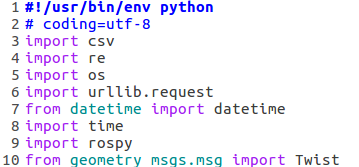
\includegraphics[width=8cm]{fig/1.png}}
		}{
			\Fonte{Elaborado pelo autor}
		}	
	\end{figure}
	
A primeira e segunda linha do código serve para utilizar caracteres especiais no código e comentários. As linhas seguintes (da 3 a 10) utilizam o método \textit{import} que serve para importar módulos para o código. Cada módulo será descrito abaixo:
\begin{description}
    \item[csv] linha 3. Serve para importar e exportar planilhas e bancos de dados;
    \item[re:] linha 4. Essa biblioteca serve para utilização de expressões regulares. Pode ser utilizado sequência de características unicode ou sequência de características 8 bits;
    \item[os:] linha 5. Serve para abrir, criar, ler e editar arquivos do sistema;
    \item[urllib.request:] linha 6. Um módulo de interface fácil para buscar dados em sites URL;
    \item[datetime:] linha 7. Manipula data e hora de forma simples ou complexa;
    \item[time:] linha 8. Função que recebe hora e data do sistema;
    \item[rospy:] linha 9. É uma biblioteca para \textit{python} que permite aos programadores terem acesso aos tópicos, serviços e parâmetros do \textit{ROS};
    \item[twist:] linha 10. Serve para enviar ou receber mensagens como pontos, vetores e valores comuns;
\end{description}

	\begin{figure}[H]
		\centering
		\Caption{Linhas de código 11 à 18 do arquivo Savefile.py}
		\UNIFORfig{}{
			\fbox{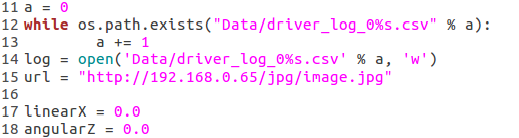
\includegraphics[width=12cm]{fig/2.png}}
		}{
			\Fonte{Elaborado pelo autor}
		}	
\end{figure}
	
Na linha 12, há um loop que procura o último driver\_log criado. Ele inicia com o valor '0', como é declarado na linha 11, e vai sendo incrementado até encontrar um valor de driver\_log que não tenha sido criado.
Na linha 15 é declarado o endereço das imagens retiradas pela câmera IP do Jaguar.

	\begin{figure}[H]
		\centering
		\Caption{Linhas de código 20 à 43 do arquivo Savefile.py}
		\UNIFORfig{}{
			\fbox{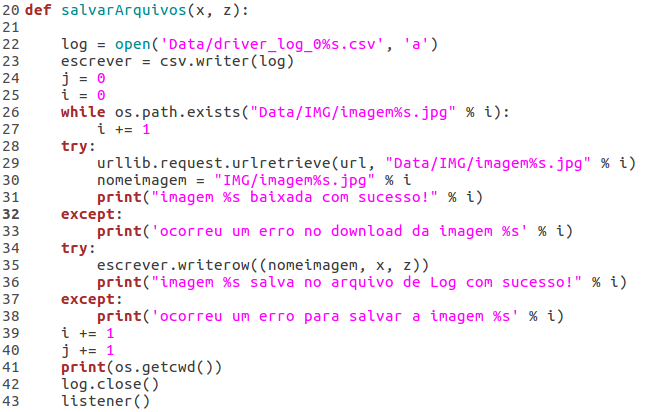
\includegraphics[width=15cm]{fig/3.png}}
		}{
			\Fonte{Elaborado pelo autor}
		}	
\end{figure}

O método salvarArquivos(), na linha 20, recebe como parâmetros a velocidade enviada para o Jaguar(variável x) e o ângulo (variável z). Primeiramente, na linha 22, será aberto o arquivo de \textit{driver\_logXX.csv} para poder escrever nele. Seguindo para a linha 26, o programa procura o valor da última imagem salva e usa um \textit{'try'} para tentar baixar a imagem fotografada pela câmera IP do Jaguar. Caso não funcione, ele exibe um erro na tela (erro nas linhas 33 e 38). 

Na linha 35 ele salva o nome da imagem, valor x e valor z dentro do arquivo csv e por último, na linha 43, ele chama o método \textit{listener()}.

	\begin{figure}[H]
		\centering
		\Caption{Linhas de código 53 à 66 do arquivo Savefile.py}
		\UNIFORfig{}{
			\fbox{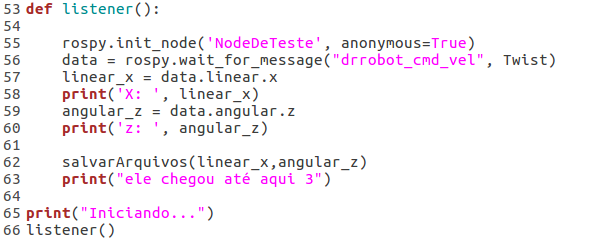
\includegraphics[width=15cm]{fig/5.png}}
		}{
			\Fonte{Elaborado pelo autor}
		}	
\end{figure}

O método \textit{listener()}, na linha 53, trata de criar um \textit{node} na rede do ROS para "ouvir" (nome utilizado para receber as mensagens de um determinado \textit{node} na rede do ROS) o \textit{node} \textit{ddrobot\_cmd\_vel} e atribuir os valores do data.linear.x e data.angular.z para o linear\_x e angular\_z, respectivamente.
Na linha 62 o método \textit{listener()} chama o método salvarArquivos() e atribui os valores de x e z aos valores linear\_x e angular\_z, respectivamente. E por último, já fora do método \textit{listener()}, esse mesmo método é chamado novamente, na linha 66, ao iniciar o programa.

\subsection{\textit{Model.py}}
\label{codigo_model}

	\begin{figure}[H]
		\centering
		\Caption{\label{model1}Linhas de código do 1 à 13 arquivo model.py}
		\UNIFORfig{}{
			\fbox{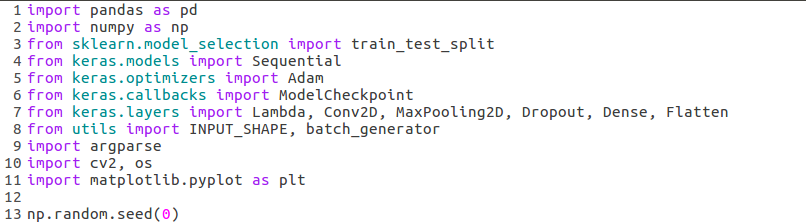
\includegraphics[width=16cm]{fig/10.png}}
		}{
			\Fonte{Elaborado pelo autor}
		}	
\end{figure}

Na Figura\ref{model1} são importadas as bibliotecas padrões que serão utilizadas no código \textit{model.py}, da linha 1 até a linha 11.

	\begin{figure}[H]
		\centering
		\Caption{\label{model2}Linhas de código do 16 à 34 arquivo model.py}
		\UNIFORfig{}{
			\fbox{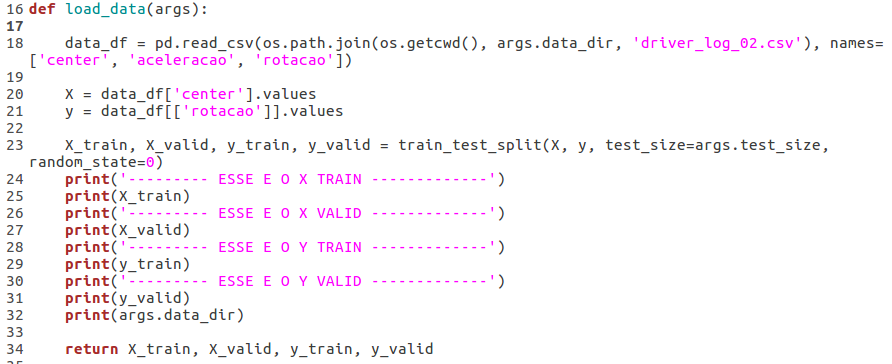
\includegraphics[width=16cm]{fig/11.png}}
		}{
			\Fonte{Elaborado pelo autor}
		}	
\end{figure}

Na linha 18 da Figura\ref{model2} a biblioteca \textit{pandas} é utilizada para abrir o arquivo \textit{.csv} criado pelo \textit{savefile.py} (\ref{sec:Savefile.py}) e transformá-lo em um \textit{dataframe} com coluna de nomes 'center', 'aceleracao' e 'rotacao'.
Na linha 20 e 21 os valores de 'center' e 'rotacao' são atribuídos as variáveis x e y, respectivamente. Na linha 23, o valor de X e y é divido em 80\% para treino (X\_train e x\_valid) e 20\% para teste (y\_train e y\_valid), no qual esse percentual está na variável test\_size.

	\begin{figure}[H]
		\centering
		\Caption{\label{model3}Linhas de código do 37 à 54 arquivo model.py}
		\UNIFORfig{}{
			\fbox{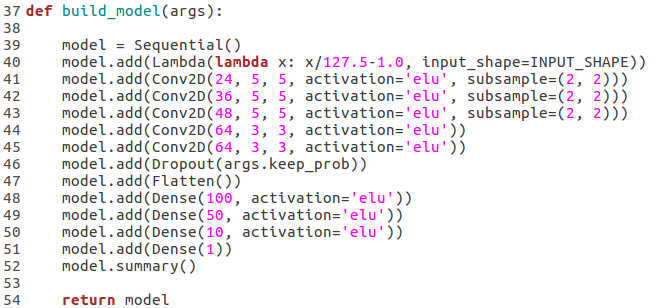
\includegraphics[width=16cm]{fig/12.png}}
		}{
			\Fonte{Elaborado pelo autor}
		}	
\end{figure}
A função da linha 37, \textit{build\_model(args)} cria a rede neural. Ela recebe como entrada um conjunto de argumentos que são declarados dentro do \textit{main()}.
Primeiramente é adicionado um espaço em branco na memória para o Keras trabalhar, na linha 39. 
Na linha 40, é adicionado uma camada de normalização de imagem. O número 127.5-1.0 foi escolhido pela comunidade de desenvolvedores depois de treinar com diferentes valores. Eles normalizam as imagens assim que são colocadas e evitam a saturação e fazem com que o gradiente funcione melhor. Ou seja, as imagens podem vim com sombras, de má qualidade. Essa função pode formatar e remodelar a imagem para trazer boas predições.
Nas linhas 40 à 45 são adicionadas 5 camadas convolucionais na rede neural. Ela recebe os seguintes argumentos: 

\begin{lstlisting}
conv2D(nb_filter, nb_row, nb_col, activation, subsample)
\end{lstlisting}

\begin{description}
    \item[nb\_filter:] Número de filtros de convolução a serem usados.
    \item[nb\_row:] Número de linhas no kernel da convolução.
    \item[nb\_col:] Número de colunas no kernel da convolução.
    \item[activation:] nome da função de ativação a ser usada. No caso, todas foram ELU:\textit{exponetial linear units}, usada para cuidar do problema gradiente de fuga
    \item[subsample:] tupla de comprimento 2. Fator pelo qual subamostra a saída.
    \item[Fonte:] \cite{kerasconv}
\end{description}
A camada de dropout, na linha 46, tem como função dar maior robustez à rede para previsões fora da amostra, buscando capturar informações populacionais ao invés de características amostrais. 
Dropout é um algoritmo relativamente novo para treinamento de redes neurais, que se fundamenta na eliminação aleatória de neurônios durante o processo de aprendizagem, para evitar a sobreadaptação aos dados (overfitting).

Na linha 47, o \textit{Flatten()} faz a preparação (achatamento) dos dados para trabalhar com series de camadas totalmente conectadas. As camadas convolucionais prepararam as imagens para serem tratadas pela rede neural. A intenção do código é achar uma relação das imagens com o \textit{steering\_angle} e o \textit{throttle}.

Da linha 48 até a linha 51 é criada a rede neural totalmente conectada. É possível observar que número de neurônios dessa rede vai reduzindo conforme a adesão de novas camadas, até chegar a um neurônio, na linha 51. 

Na linha 51 há uma função para imprimir os valores dos \textit{layers} e na 54 a função retorna o modelo criado.

	\begin{figure}[H]
		\centering
		\Caption{\label{model4}Linhas de código do 57 à 74 arquivo model.py}
		\UNIFORfig{}{
			\fbox{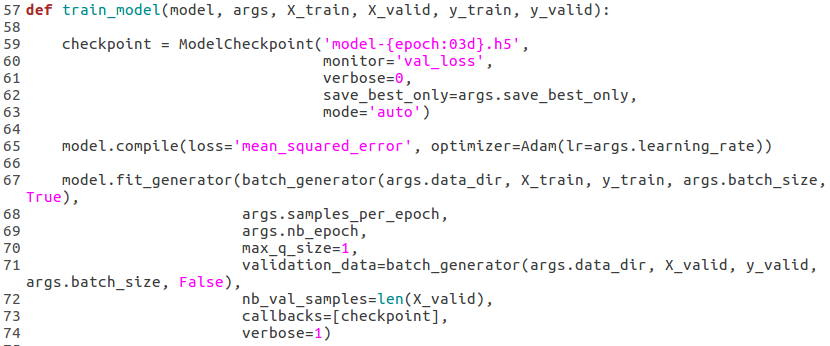
\includegraphics[width=16cm]{fig/13.png}}
		}{
			\Fonte{Elaborado pelo autor}
		}	
\end{figure}

A função \textit{train\_model()}, linha 57 da Figura\ref{model4}, tem como função treinar o modelo criado. Na linha 59, há um método que salva um modelo a cada \textit{epoch} (quantidade de vezes que o conjunto será treinado), caso ele tenha um \textit{'val\_loss'} menor que o anterior.

O Compilador do modelo, na linha 65, utiliza o método \textit{'mean\_squared\_error'}, que calcula a diferença entre o quadrado do valor esperado e o quadrado do valor obtido e tira a média de todos os valores obtidos para achar o erro. Esse método utiliza o otimizador Adam, que é um gradiente de descida.

\[\sum_{1}^{n}\frac{(valor\_real - valor\_obtido)^{2}}{n}\]

Na linha 67, o \textit{mode.fit\_generator} faz o treinamento do modelo. Ele utiliza o método \textit{batch\_generator()} do arquivo \textit{utils.py} e argumentos do \textit{main()} para fazer o treinamento e o \textit{checkpoint} da linha 59 para salvar o modelo treinado.

	\begin{figure}[H]
		\centering
		\Caption{\label{model5}Linhas de código do 77 à 80 arquivo model.py}
		\UNIFORfig{}{
			\fbox{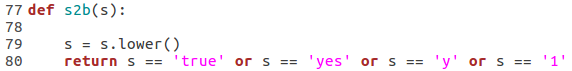
\includegraphics[width=14cm]{fig/14.png}}
		}{
			\Fonte{Elaborado pelo autor}
		}	
\end{figure}

O método \textit{s2b(s)} da Figura\ref{model5} é um simples método utilizado no \textit{main()} para converter \textit{strings} em valores booleanos.

	\begin{figure}[H]
		\centering
		\Caption{\label{model6}Linhas de código do 83 à 108 arquivo model.py}
		\UNIFORfig{}{
			\fbox{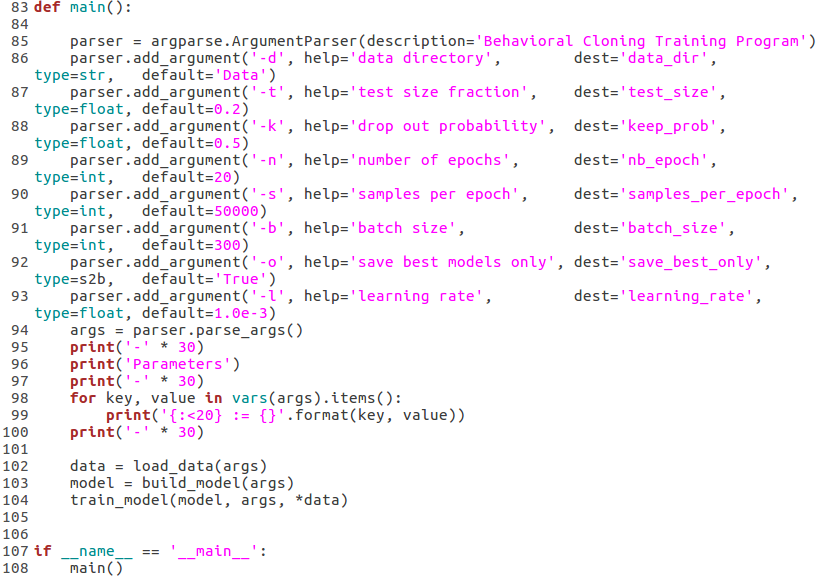
\includegraphics[width=16cm]{fig/15.png}}
		}{
			\Fonte{Elaborado pelo autor}
		}	
\end{figure}

A função inicial do \textit{main()} da Figura\ref{model6}, linha 83,  é a criação de uma instância do \textit{ArgumentParser}, a \textit{parser}, e atribuição dos seus argumentos, da linha 86 a 93.
Após a exibição dos parâmetros na tela, da linha 95 até 100, a função \textit{main()} chama as funções \textit{load\_data(args)}, \textit{build\_lode(args)} e \textit{train\_model(model, args, *data)} com os argumentos criados nessa função.

Ao final, na linha 108, a função \textit{main()} é chamada dentro do loop de verificação para inicar o programa.

\subsection{\textit{utils.py}}
\label{sec:utils.py}

	\begin{figure}[H]
		\centering
		\Caption{\label{utils1}Linhas de código do 1 à 7 arquivo utils.py}
		\UNIFORfig{}{
			\fbox{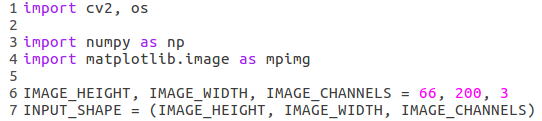
\includegraphics[width=16cm]{fig/16.png}}
		}{
			\Fonte{Elaborado pelo autor}
		}	
\end{figure}
A Figura\ref{utils1} mostra basicamente as bibliotecas que são importadas para esse arquivo( no caso, \textit{OpenCV}, \textit{Miscellaneous operating system interfaces}, \textit{Numpy} e \textit{Matplot}, da linha 1 até a linha 4), atribui valores para as variáveis \textit{IMAGE\_HEIGHT}, \textit{IMAGE\_WIDTH} e \textit{\IMAGE\_CHANNELS} e coloca todas esse valores na tupla \textit{INPUT\_SHAPE}.


\begin{figure}[H]
	\centering
	\Caption{\label{utils2}Linhas de código do 10 à 39 arquivo utils.py}
	\UNIFORfig{}{
		\fbox{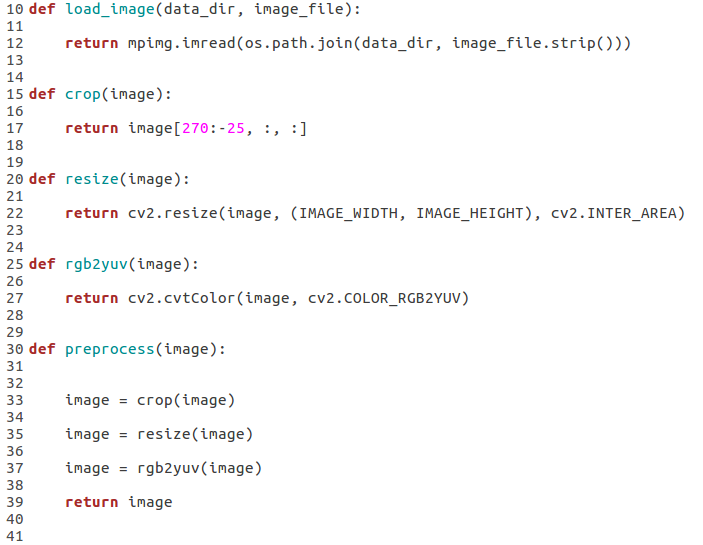
\includegraphics[width=16cm]{fig/17.png}}
	}{
		\Fonte{Elaborado pelo autor}
	}	
\end{figure}

Na Figura\ref{utils2} há cinco métodos, onde o primeiro tem a função de carregar a imagem para o programa (método \textit{load\_image}, linha 10). Os métodos \textit{crop}, \textit{resize} e \textit{rgb2yuv} (na linha 15, 20 e 25, respectivamente) fazem edições nas imagens e o método final, \textit{preprocess(imagem)}, na linha 30, trata de chamar os métodos de edição de imagem.

\begin{figure}[H]
	\centering
	\Caption{\label{utils3}Linhas de código do 42 à 93 arquivo utils.py}
	\UNIFORfig{}{
		\fbox{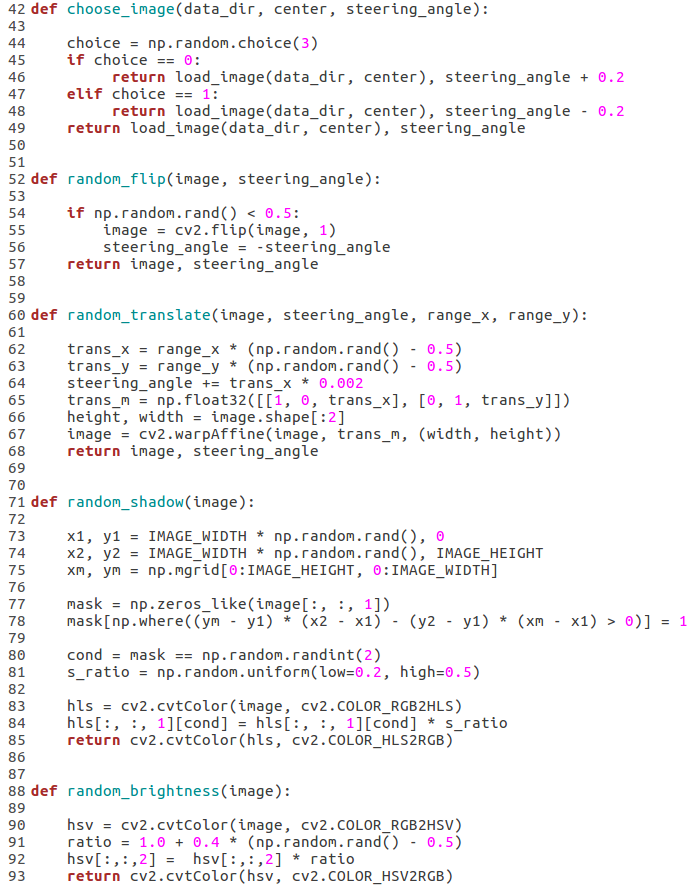
\includegraphics[width=16cm]{fig/18.png}}
	}{
		\Fonte{Elaborado pelo autor}
	}	
\end{figure}

Os métodos utilizados na Figura\ref{utils3} servem para complementar o método \textit{augument()}, modificando a imagem de diversas maneiras.
\begin{description}
    \item[choose\_image(data\_dir, center, steering\_angle):] Linha 42. Escolha aleatoriamente uma imagem e modifica o ângulo de direção.
    \item[random\_flip(image, steering\_angle):] Linha 52. Gira aleatoriamente a imagem para a esquerda ou para a direita, ajustando o ângulo de direção.
    \item[random\_translate(image, steering\_angle, range\_x, range\_y):] Linha 60. Faz uma translação aleatória na imagem.
    \item[random\_shadow(image):] Linha 71. Gera e adiciona sombra aleatória.
    \item[random\_brightness(image):] Linha 88. Ajusta aleatoriamente o brilho da imagem.
\end{description}

\begin{figure}[H]
	\centering
	\Caption{\label{utils4}Linhas de código do 96 à 103 arquivo utils.py}
	\UNIFORfig{}{
		\fbox{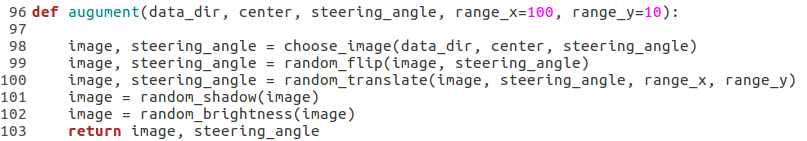
\includegraphics[width=16cm]{fig/19.png}}
	}{
		\Fonte{Elaborado pelo autor}
	}	
\end{figure}

O método \textit{augument()} da linha 96 da Figura\ref{utils4} utiliza os métodos descritos na Figura\ref{utils3}, da linha 42 à 88, para gerar uma imagem diferente das imagens capturadas. Aumentando o número de imagens melhora a previsão da rede neural.

\begin{figure}[H]
	\centering
	\Caption{\label{utils5}Linhas de código do 96 à 103 arquivo utils.py}
	\UNIFORfig{}{
		\fbox{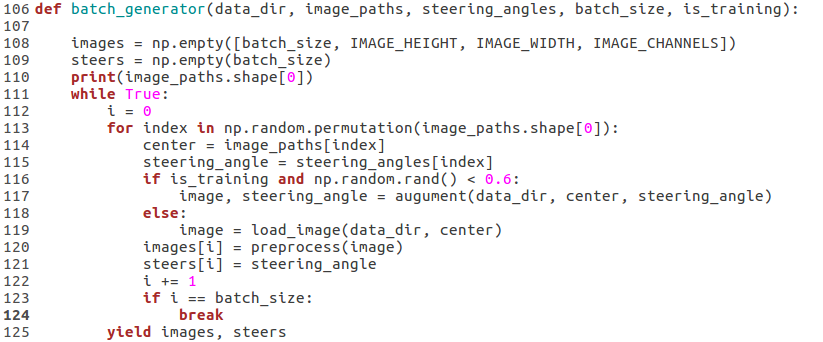
\includegraphics[width=16cm]{fig/20.png}}
	}{
		\Fonte{Elaborado pelo autor}
	}	
\end{figure}

A função \textit{batch\_generator} da Figura\ref{utils5} é gerar imagem de treinamento modificada, fornecer o caminho da imagem e dos ângulos de direção e associar a dois \textit{arrays}: \textit{images} e \textit{steers}. Nesse função é possível escolher se a modificação será feita pelo método \textit{augument()}, citado na Figura\ref{utils4} ou pelo método \textit{preprocess()}, da Figura\ref{utils2}. Para o treinamento da rede neural do projeto, é utilizado o método \textit{augument()} e o método \textit{preprocess()} serve para fazer a validação dos dados treinados.

\subsection{\textit{drive.py}}
\label{sec:drive.py}

\begin{figure}[H]
	\centering
	\Caption{Linhas de código do 1 à 18 arquivo drive.py}
	\UNIFORfig{}{
		\fbox{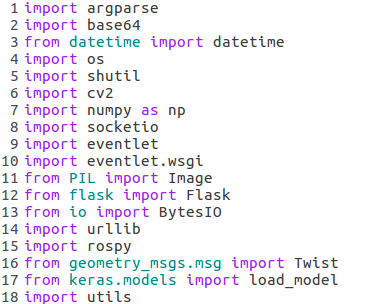
\includegraphics[width=12cm]{fig/6.png}}
	}{
		\Fonte{Elaborado pelo autor}
	}	
\end{figure}

Na linha 1 até a linha 18 do arquivo \textit{drive.py} são importadas as bibliotecas essenciais para o funcionamento do programa.

\begin{figure}[H]
	\centering
	\Caption{{\label{figura 7}}Linhas de código do 20 à 29 arquivo drive.py}
	\UNIFORfig{}{
		\fbox{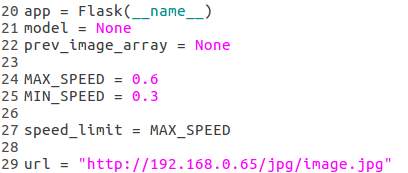
\includegraphics[width=12cm]{fig/7.png}}
	}{
		\Fonte{Elaborado pelo autor}
	}	
\end{figure}

Na Figura\ref{figura 7}, da linha 20 até á 25, são declaradas as variáveis a serem utilizadas no restante do programa. Na linha 27 a velocidade máxima é limitada ao valor de \textit{MAX\_SPEED} e na linha 29 o link da câmera IP é atribuído à variável \textit{url}.
\begin{figure}[H]
	\centering
	\Caption{{\label{figura 8}}Linhas de código do 20 à 29 arquivo drive.py}
	\UNIFORfig{}{
		\fbox{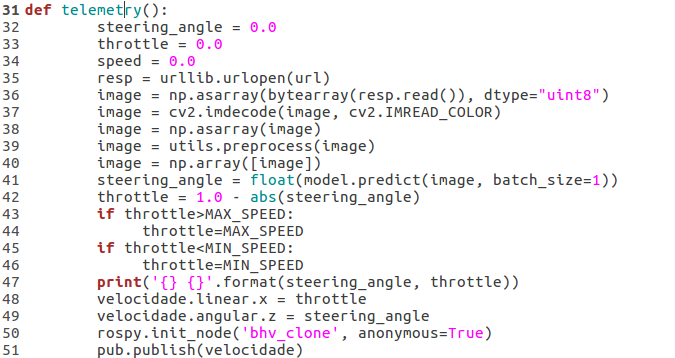
\includegraphics[width=14cm]{fig/8.png}}
	}{
		\Fonte{Elaborado pelo autor}
	}	
\end{figure}

Na linha 31, a função \textit{telemetry()} da Figura\ref{figura 8} começa zerando os valores das variáveis \textit{steering\_angle, throttle} e \textit{speed}. Na linha 35 ele recebe a imagem capturada pelo Jaguar e faz a tratamento dela com os mesmos valores utilizados para criar o modelo. Na linha 41 é criado a previsão para a imagem analisada e salva na instância \textit{steering\_angle}. O \textit{throttle} recebe o valor de 1 menos o módulo do ângulo de direção para diminuir a velocidade conforme ele gira. As linhas 43 e 45 garantem que o valor de velocidade seja sempre menor que valor máximo.

Ao final da função \textit{telemetry()} os valores de \textit{steering\_angle} e \textit{throttle} são imprimidos na tela e colocados nas variáveis \textit{velocidade.linear.x} e \textit{velocidade.angular.z} para finalmente serem publicados no  \textit{Node} do Jaguar.

\begin{figure}[H]
	\centering
	\Caption{{\label{figura 9}}Linhas de código do 53 à 74 arquivo drive.py}
	\UNIFORfig{}{
		\fbox{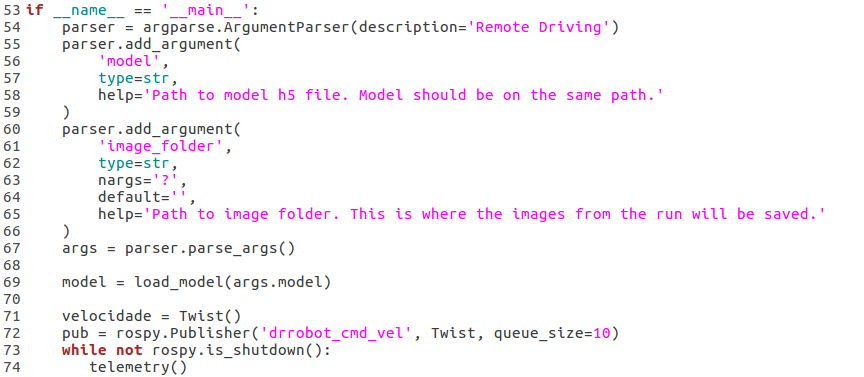
\includegraphics[width=16cm]{fig/9.png}}
	}{
		\Fonte{Elaborado pelo autor}
	}	
\end{figure}

Dentro da função \textit{main()}, da linha 54 até a linha 67, são criados os argumentos de localização do modelo e da pasta de imagens. Essa localização tem que ser fornecida pelo usuário no momento de execução do programa. A instância velocidade recebe então a função \textit{Twist()} e é criado, na linha 72, um tópico chamado \textit{pup} para a publicação de mensagens no \textit{Node} do Jaguar. Na linha 73, enquanto o \textit{Node} do \textit{Jaguar} estiver ligado a função \textit{main()} irá continuar chamando a função \textit{telemetry()}.
	\chapter{Resultados}

\section{PRIMEIRO TESTE}
\label{primeiro_teste}
O primeiro teste do projeto foi realizado na pista de atletismo da Unifor, no dia 8 de dezembro.
Logo ao chegar na pista de atletismo deparamos com o primeiro problema: a extensão não era grande o suficiente para atingir todo o percurso que escolhemos para treinar o Jaguar. Pedimos então aos auxiliares por uma nova extensão que foi entregue em pouco tempo. O jaguar foi treinado em apenas uma parte da pista, indo e voltando duas vezes. o caminho percorrido é mostrado na figura \ref{pistaunifor}.

	\begin{figure}[H]
		\centering
		\Caption{\label{pistaunifor} Vista Aérea da Pista da Unifor}
		\UNIFORfig{}{
			\fbox{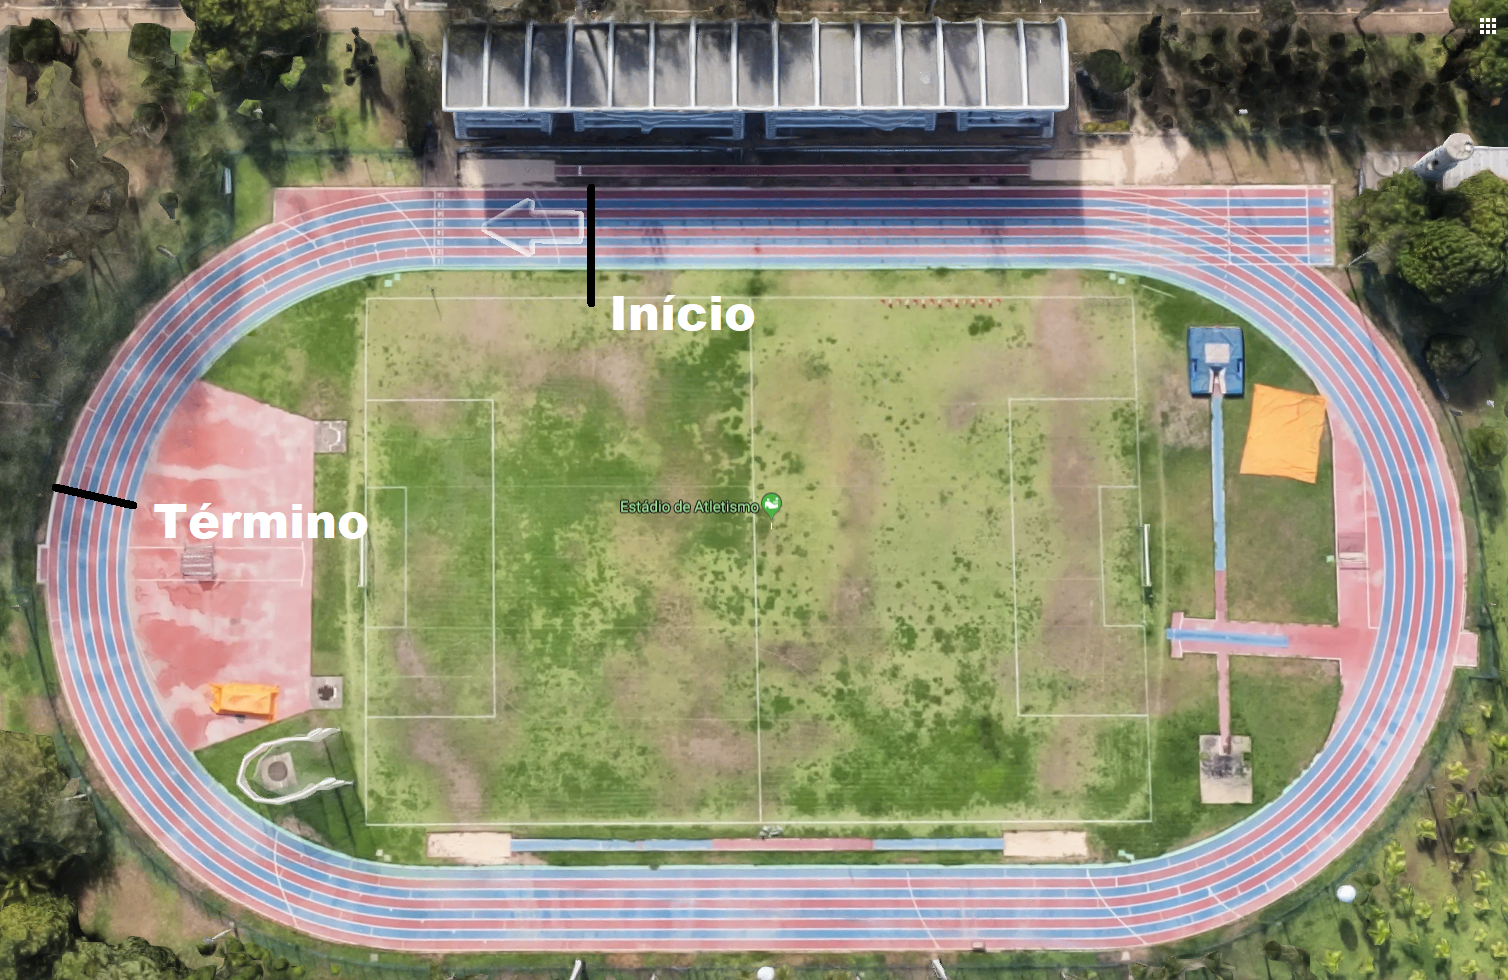
\includegraphics[width=16cm]{figuras/PistaUnifor.png}}
		}{
			\Fonte{\cite{pistaunifor}}
		}	
\end{figure}

Foram obtidas 977 imagens, o que ainda é muito pouco para criação de um modelo adequado para esse tipo de trabalho. Essas Imagens foram obtidas pela câmera do jaguar usando o programa \textit{savefile.py} enquanto um aluno pilotava o robô. As imagens são tiradas a cada movimento novo realizado no \textit{Joystick}. Na imagem \ref{jaguarelog} podemos ver a esquerda um exemplo de imagem capturada pela câmera do jaguar e a direta o resultado do terminal de execução do programa \textit{savefile.py}.

	\begin{figure}[H]
		\centering
		\Caption{\label{jaguarelog}Exemplo de Imagem capturada pelo câmera do Jaguar e o Terminal do programa \textit{Savefile.py}}
		\UNIFORfig{}{
			\fbox{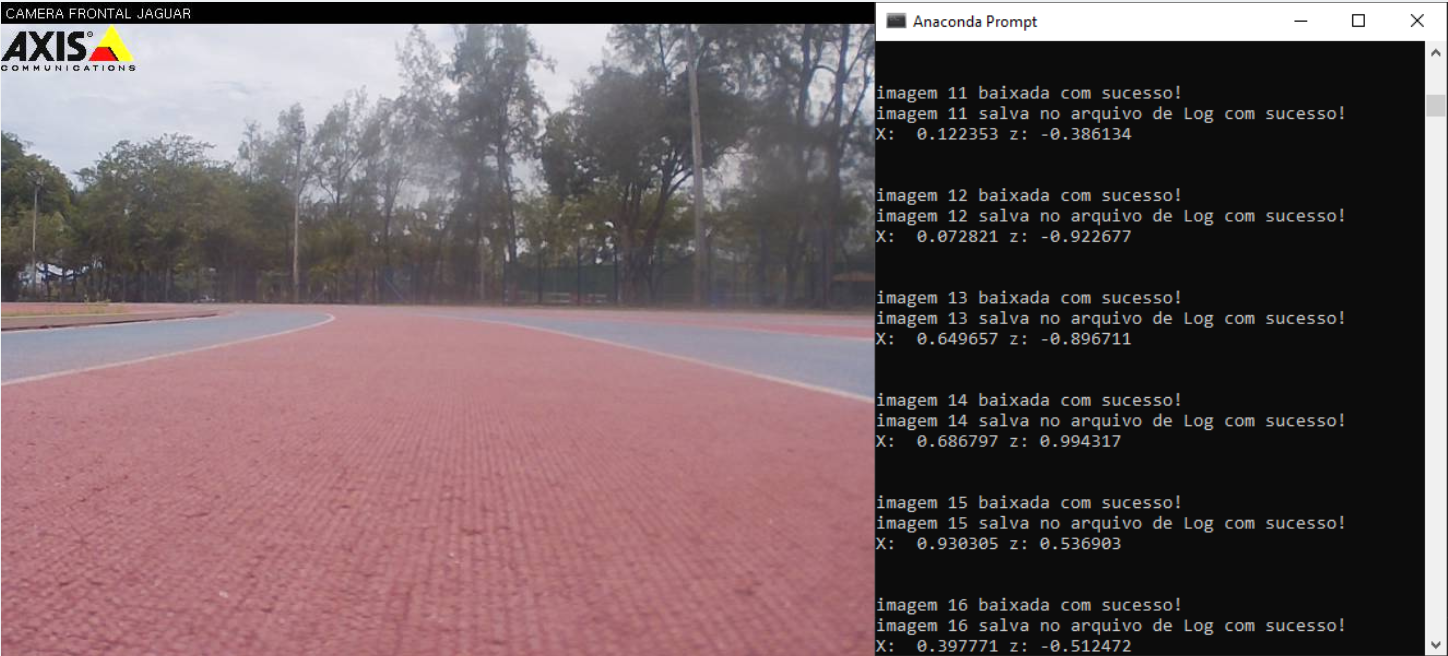
\includegraphics[width=16cm]{figuras/JaguarELog.png}}
		}{
			\Fonte{Elaborada pelo autor}
		}	
\end{figure}

O programa python tem acesso as imagens do Jaguar pelo IP de sua câmera. Ao final da captura das imagens, foi executado o programa \textit{model.py} que trata de criar o modelo de testes pro Jaguar, resultado no arquivo \textit{model-XXX.h5}, onde o "XXX" é o número do modelo da vez.

O programa \textit{model.py} tem o diretório com acesso a todas as imagens capturadas e o \textit{driver\_log} criado, caso não tenha sido mudado de lugar. Mas antes de criar o modelo, é feito um tratamento na imagem, com o auxílio do arquivo \textit{util.py}, para que seja processada com mais facilidade pela rede neural. O primeiro processo consiste em cortar o céu da imagem, que não será útil para o tratamento pela rede neural(função \textit{crop()}, letra 'B'); reduzir o tamanho da imagem, o suficiente para ainda sim conseguir ser tratada pela rede neural e não perder nenhuma característica importante (função \textit{resize()}, letra 'C'); por último, muda as cores da imagem de rgb (o tradicional formato de imagem colorida) para yuv (um formato mais simples de imagem utilizando menos cores e de processamento mais fácil) (função \textit{rgb2yuv()}, letra 'D'). Os três processos são mostrados na figura \ref{combo}, onde a primeira imagem (letra 'A') é o exemplo utilizado para realizar o processo.

	\begin{figure}[H]
		\centering
		\Caption{\label{combo} Tratamento da Imagem}
		\UNIFORfig{}{
			\fbox{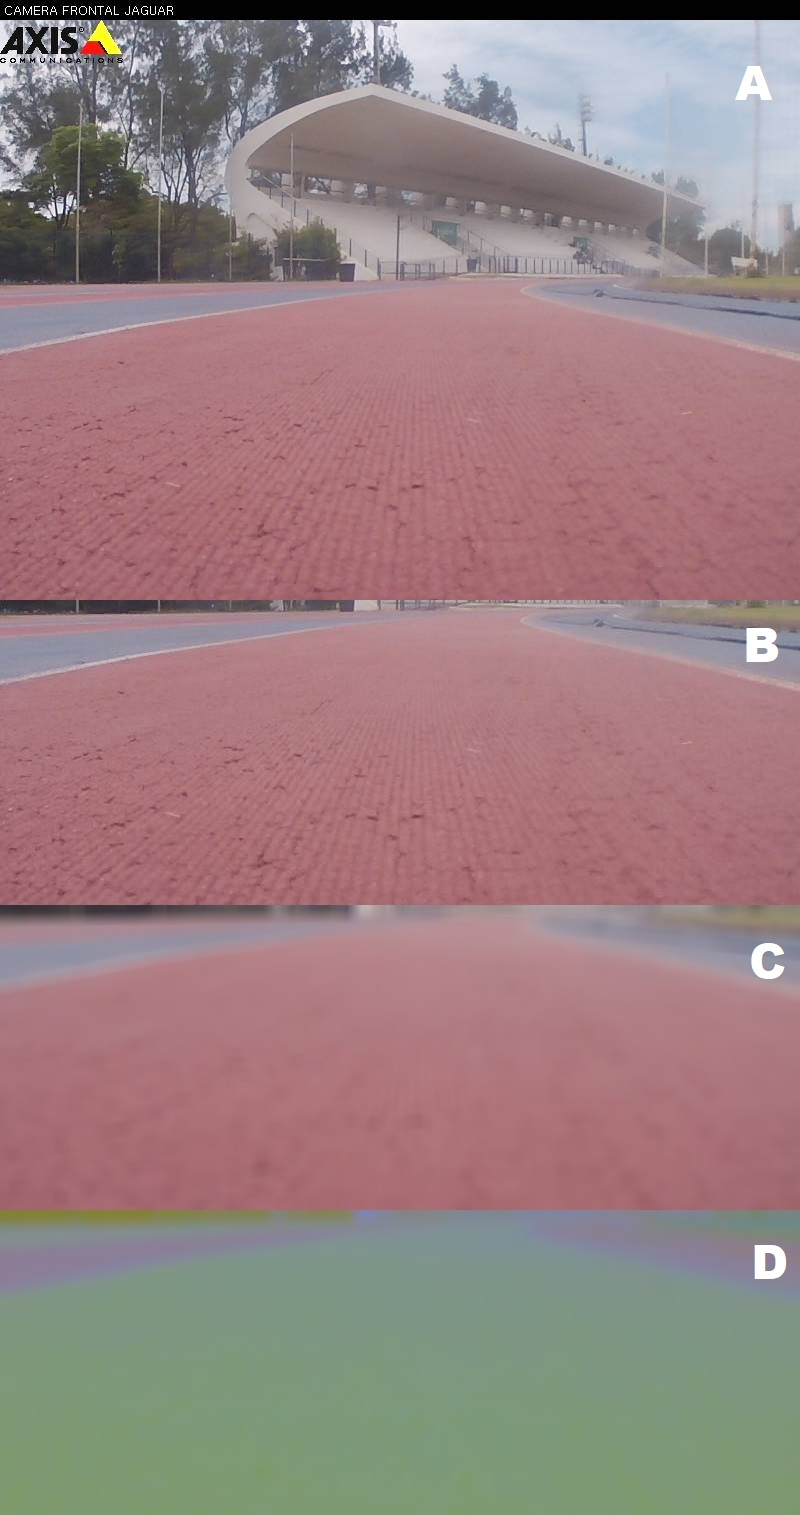
\includegraphics[width=10cm]{figuras/combo.jpg}}
		}{
			\Fonte{Elaborada pelo autor}
		}	
\end{figure}

Depois da imagem tratada, é feito a criação dos modelos de rede neural, no qual o melhor será aquela com o menor \textit{val\_loss}. Para isso, é preciso modificar alguns parâmetros dentro do \textit{model.py}: \textit{np\_epoch} (defini o número de épocas de criação do modelo, ou seja, quantas vezes ele será treinado com aqueles padrões), \textit{sample\_per\_epoch} (quantidade de imagens por época) e \textit{batch\_size} (tamanho do lote de imagem de treinamento por vez). Normalmente a criação do modelo pode levar horas e exigir muito processamento do computador. Os parâmetros utilizado para cada treinamento estão na tabela \ref{parametros1}.

\begin{table}[H]
\centering
\caption{ Tabela de parâmetros do primeiro para primeira pista}
\label{parametros1}
\begin{tabular}{|l|l|l|l|}
\hline
\textbf{Treinamento} & \textbf{nb\_epoch} & \textbf{samples\_per\_epoch} & \textbf{batch\_size} \\ \hline
1º        & 5         & 5000                & 100         \\ 
2º        & 10        & 5000                & 100         \\ 
3º        & 5         & 10000               & 100         \\ 
4º        & 10        & 10000               & 100         \\ 
5º        & 15        & 10000               & 100         \\ 
6º        & 15        & 20000               & 150         \\ \hline
\end{tabular}
\end{table}

O \textit{model.py} está programado para criar o próximo modelo somente se houver um erro menor que o modelo anterior. Ás vezes ele cria somente um modelo pois o primeiro foi o melhor de todos, outras vezes ele cria vários modelos. Isso depende de cada caso.
No sábado seguinte, foi colocado para testar o último modelo criado, o \textit{model-009.h5} e, para a surpresa de todos, ele funcionou perfeitamente, sem a necessidade de testar nenhum outro modelo. Segue abaixo o valor do \textit{loss}:

\begin{lstlisting}
loss: 0.0937 - val\_loss: 0.0564
\end{lstlisting}

Com o notebook conectado ao Jaguar, o Programa \textit{drive.py} foi executado juntamente com o \textit{model-009.h5} e, com apenas esse primeiro modelo, foi possível colocar a plataforma para percorrer a pista de atletismo nos dois sentido. A figura \ref{testejaguar} Mostra o teste realizado na pista no qual o notebook está no chão, ao lado do robô.

	\begin{figure}[H]
		\centering
		\Caption{\label{testejaguar}Teste do Jaguar}
		\UNIFORfig{}{
			\fbox{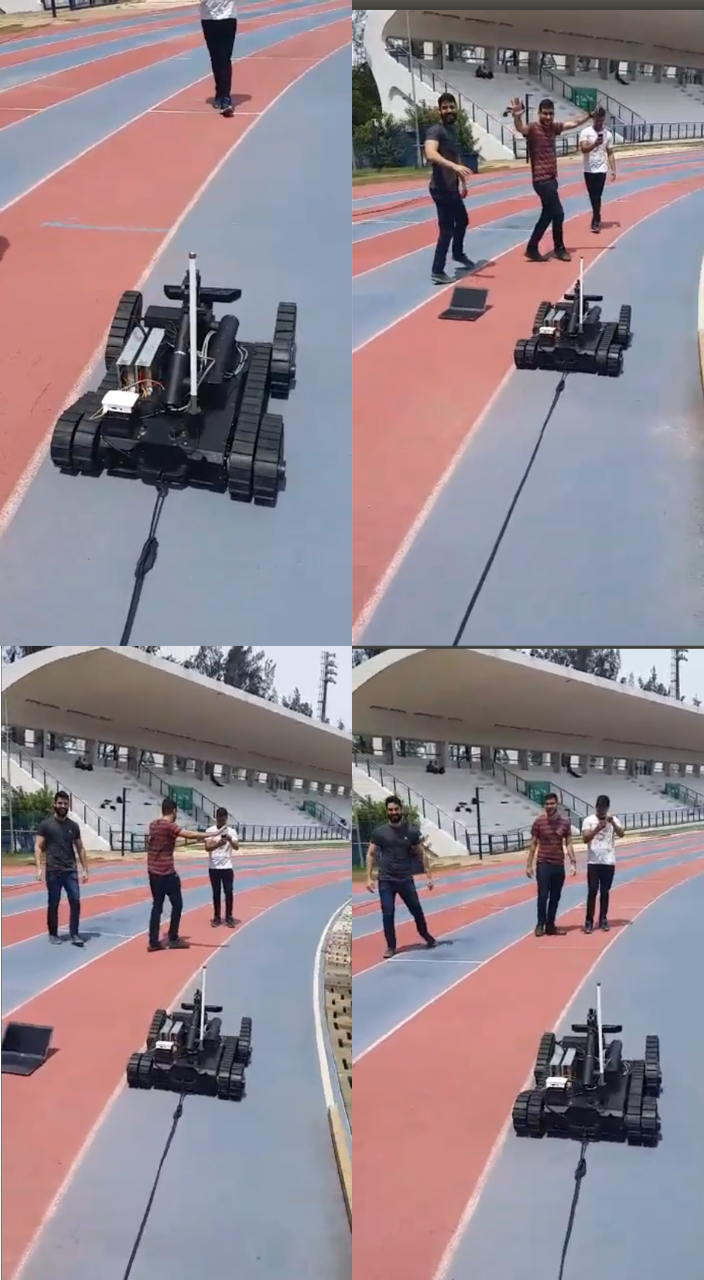
\includegraphics[height=14cm]{figuras/testejaguar.png}}
		}{
			\Fonte{Elaborado pelo autor}
		}	
\end{figure}


Em alguns momentos o Jaguar foi deslocado um pouco da sua rota. Mesmo assim ele consegue retornar a pista. Os resultados foram impressionantes, principalmente pelo fato das inúmeras limitações para o desenvolvimento do projeto.

\section{SEGUNDO TESTE}
\label{segundo}

Para validação do trabalho, é preciso que o Jaguar consiga treinar e percorrer em outros circuitos. O segundo teste foi feita na sala L4 com o formato de pista representado na figura \ref{circuito}:

	\begin{figure}[H]
		\centering
		\Caption{\label{circuito} Circuito da pista 2}
		\UNIFORfig{}{
			\fbox{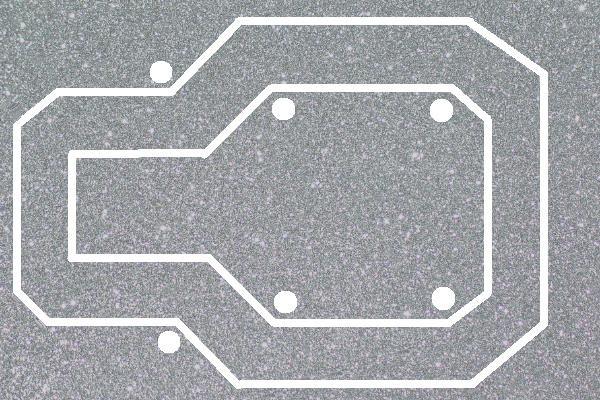
\includegraphics[width=14cm]{figuras/pistaL4.png}}
		}{
			\Fonte{Elaborado pelo autor}
		}	
\end{figure}

O segundo teste foi o mais trabalhoso. Ele foi realizado no laboratório L4 e a pista teve que ser refeita três vezes. A primeira foi a mais simples, feita de fita adesiva. Ela é mostrada na figura \ref{pista1}.

	\begin{figure}[H]
		\centering
		\Caption{\label{pista1} Primeira Pista da L4}
		\UNIFORfig{}{
			\fbox{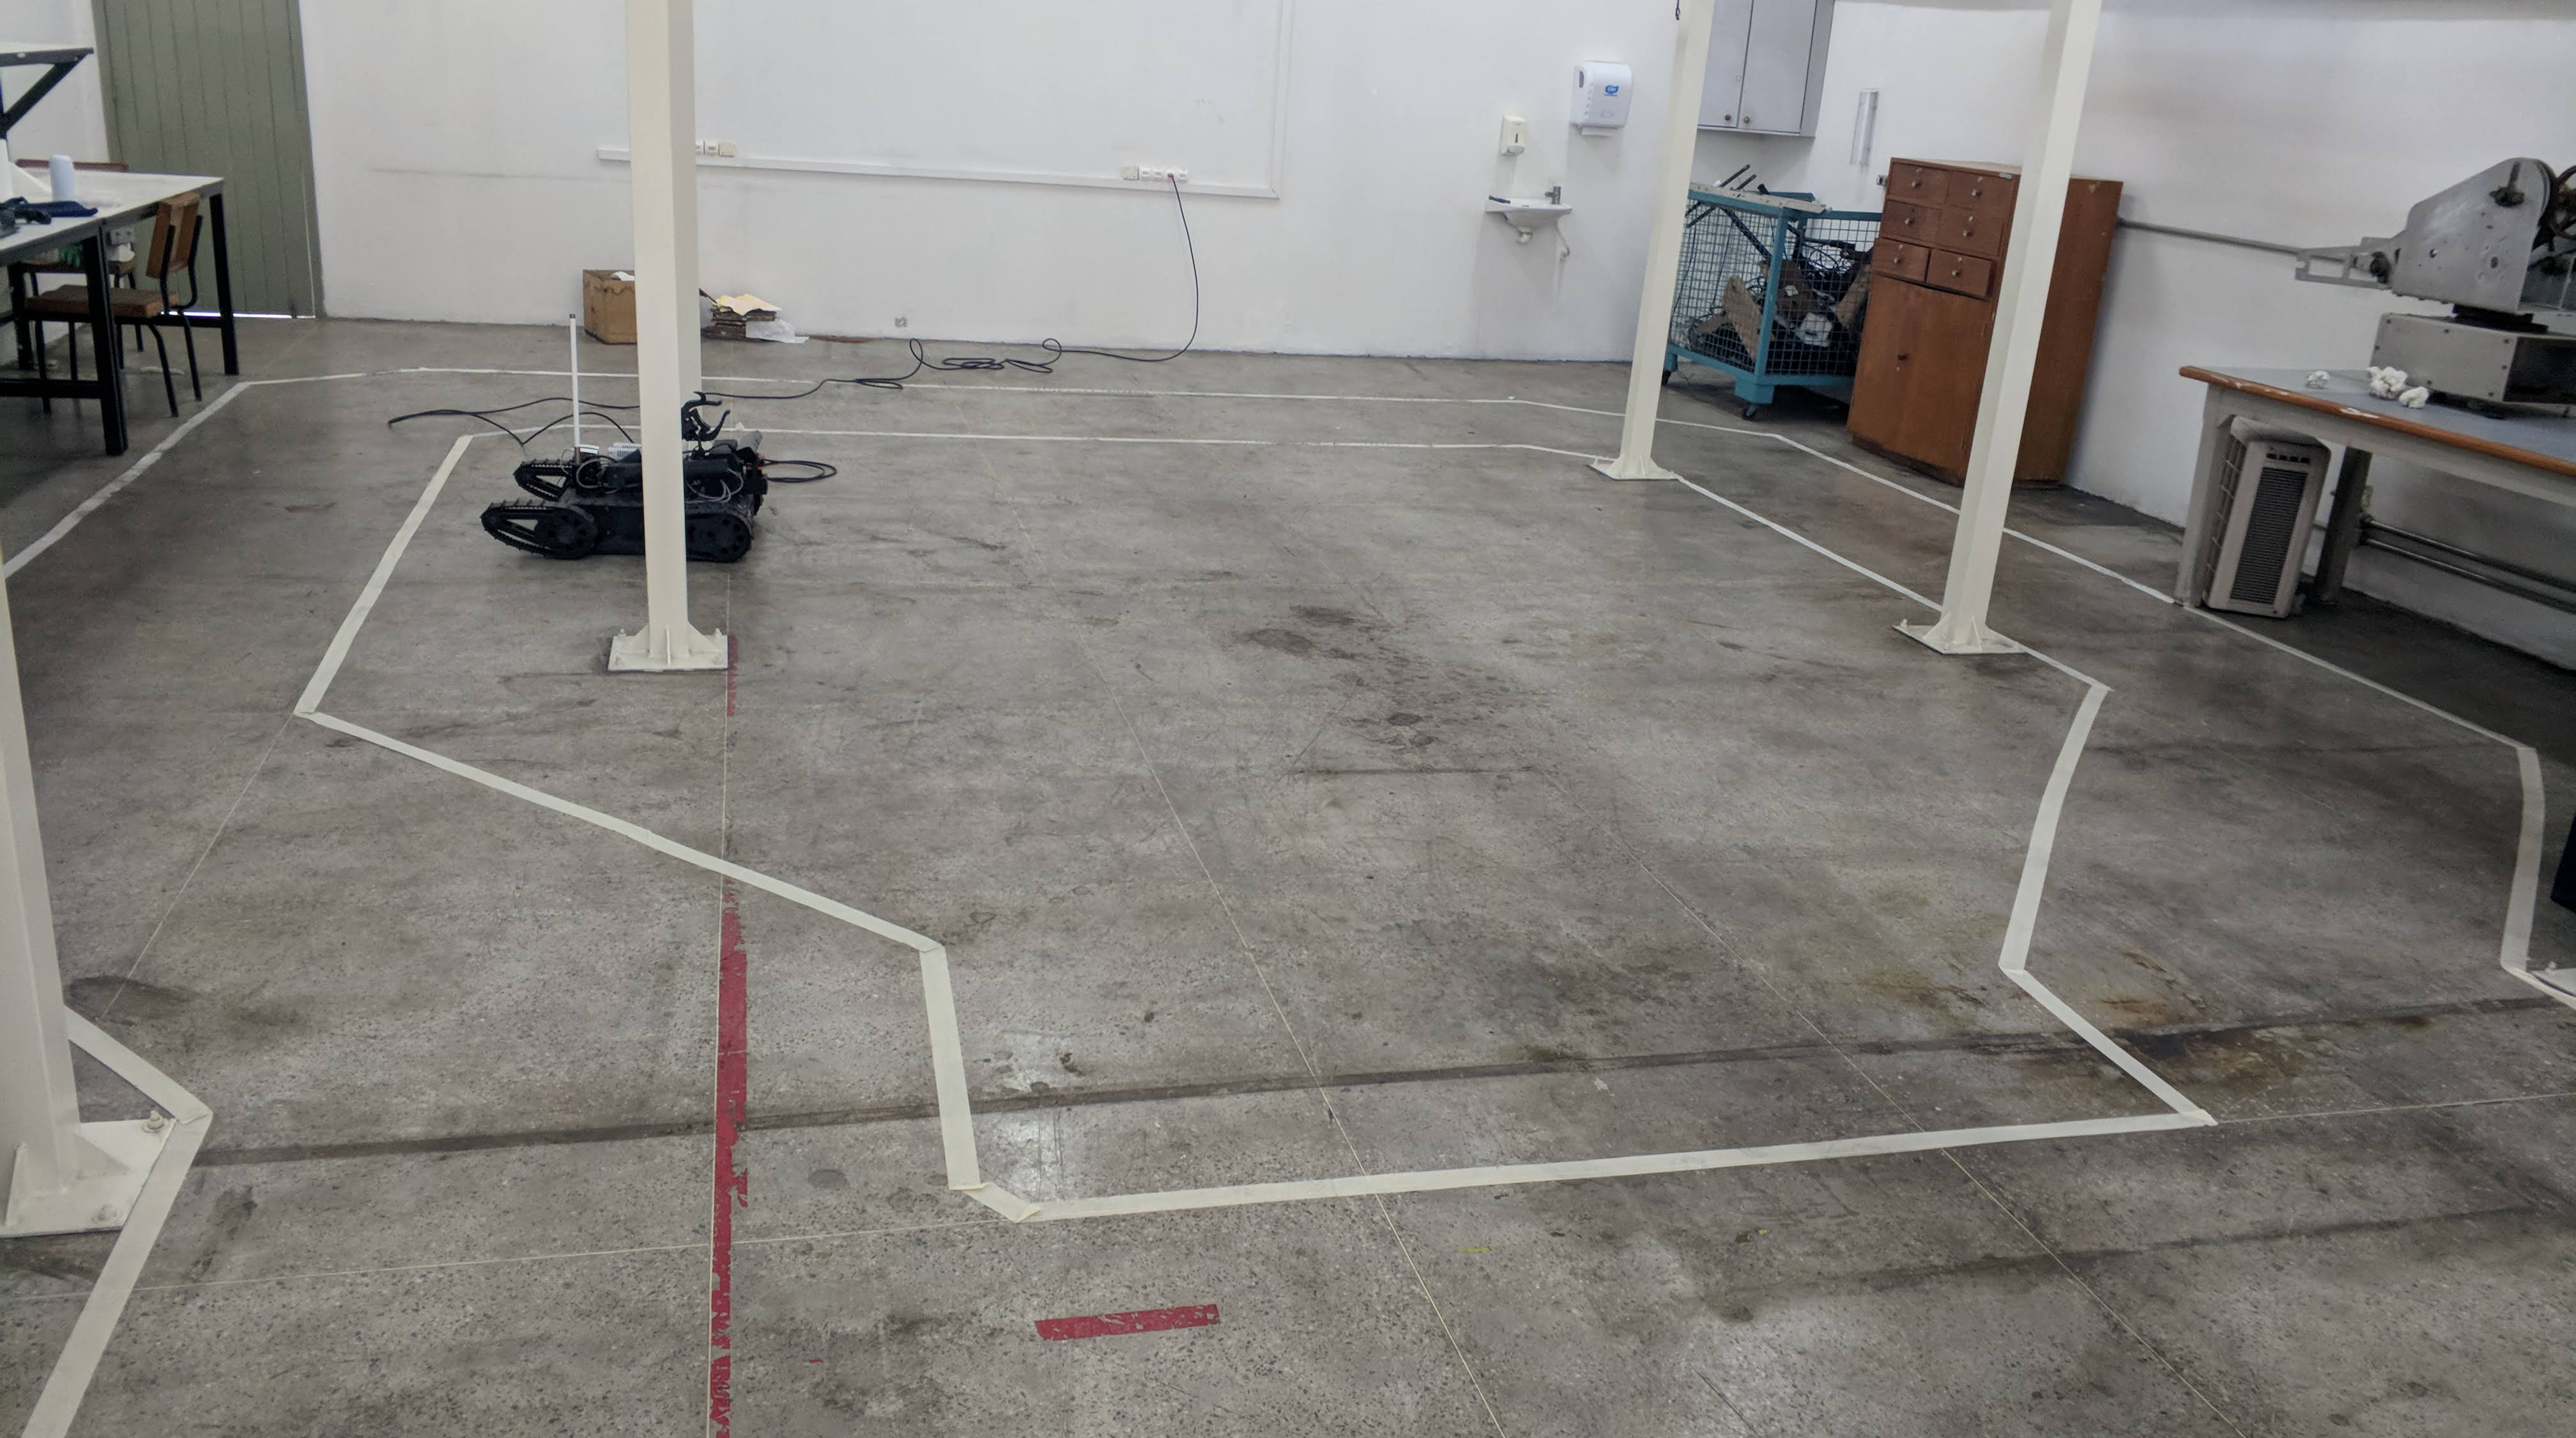
\includegraphics[width=15cm]{figuras/pista1.jpg}}
		}{
			\Fonte{Elaborado pelo autor}
		}	
\end{figure}

O primeiro grande desafio enfrentado foi desenhar um modelo de pista no qual o Jaguar conseguisse visualizar. A fita adesiva, muito fina, não se destacava o suficiente no chão de cinza da L4. Mesmo com várias tentativas e vários modelos criados o Jaguar conseguia no máximo seguir por uma reta ou uma curva simples, mas logo se perdia. A imagem \ref{imagem1} mostra um exemplo de imagem capturada pelo Jaguar nessa pista.

	\begin{figure}[H]
		\centering
		\Caption{\label{imagem1} Imagem Capturada pela câmera do Jaguar}
		\UNIFORfig{}{
			\fbox{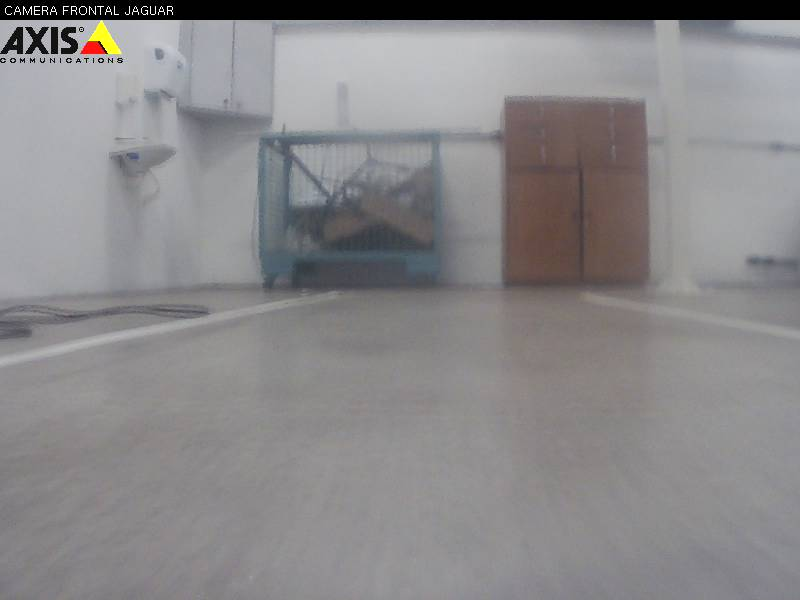
\includegraphics[width=14cm]{figuras/imagem1242.jpg}}
		}{
			\Fonte{Elaborado pelo autor}
		}	
\end{figure}


Mediante o problema de largura da pista, foi criado uma nova seguindo o mesmo modelo da anterior, porém com as bordas mais largas e feita de fita adesiva e papel toalha. Segue a pista na Figura \ref{pista2}:

	\begin{figure}[H]
		\centering
		\Caption{\label{pista2} Segunda Pista da L4}
		\UNIFORfig{}{
			\fbox{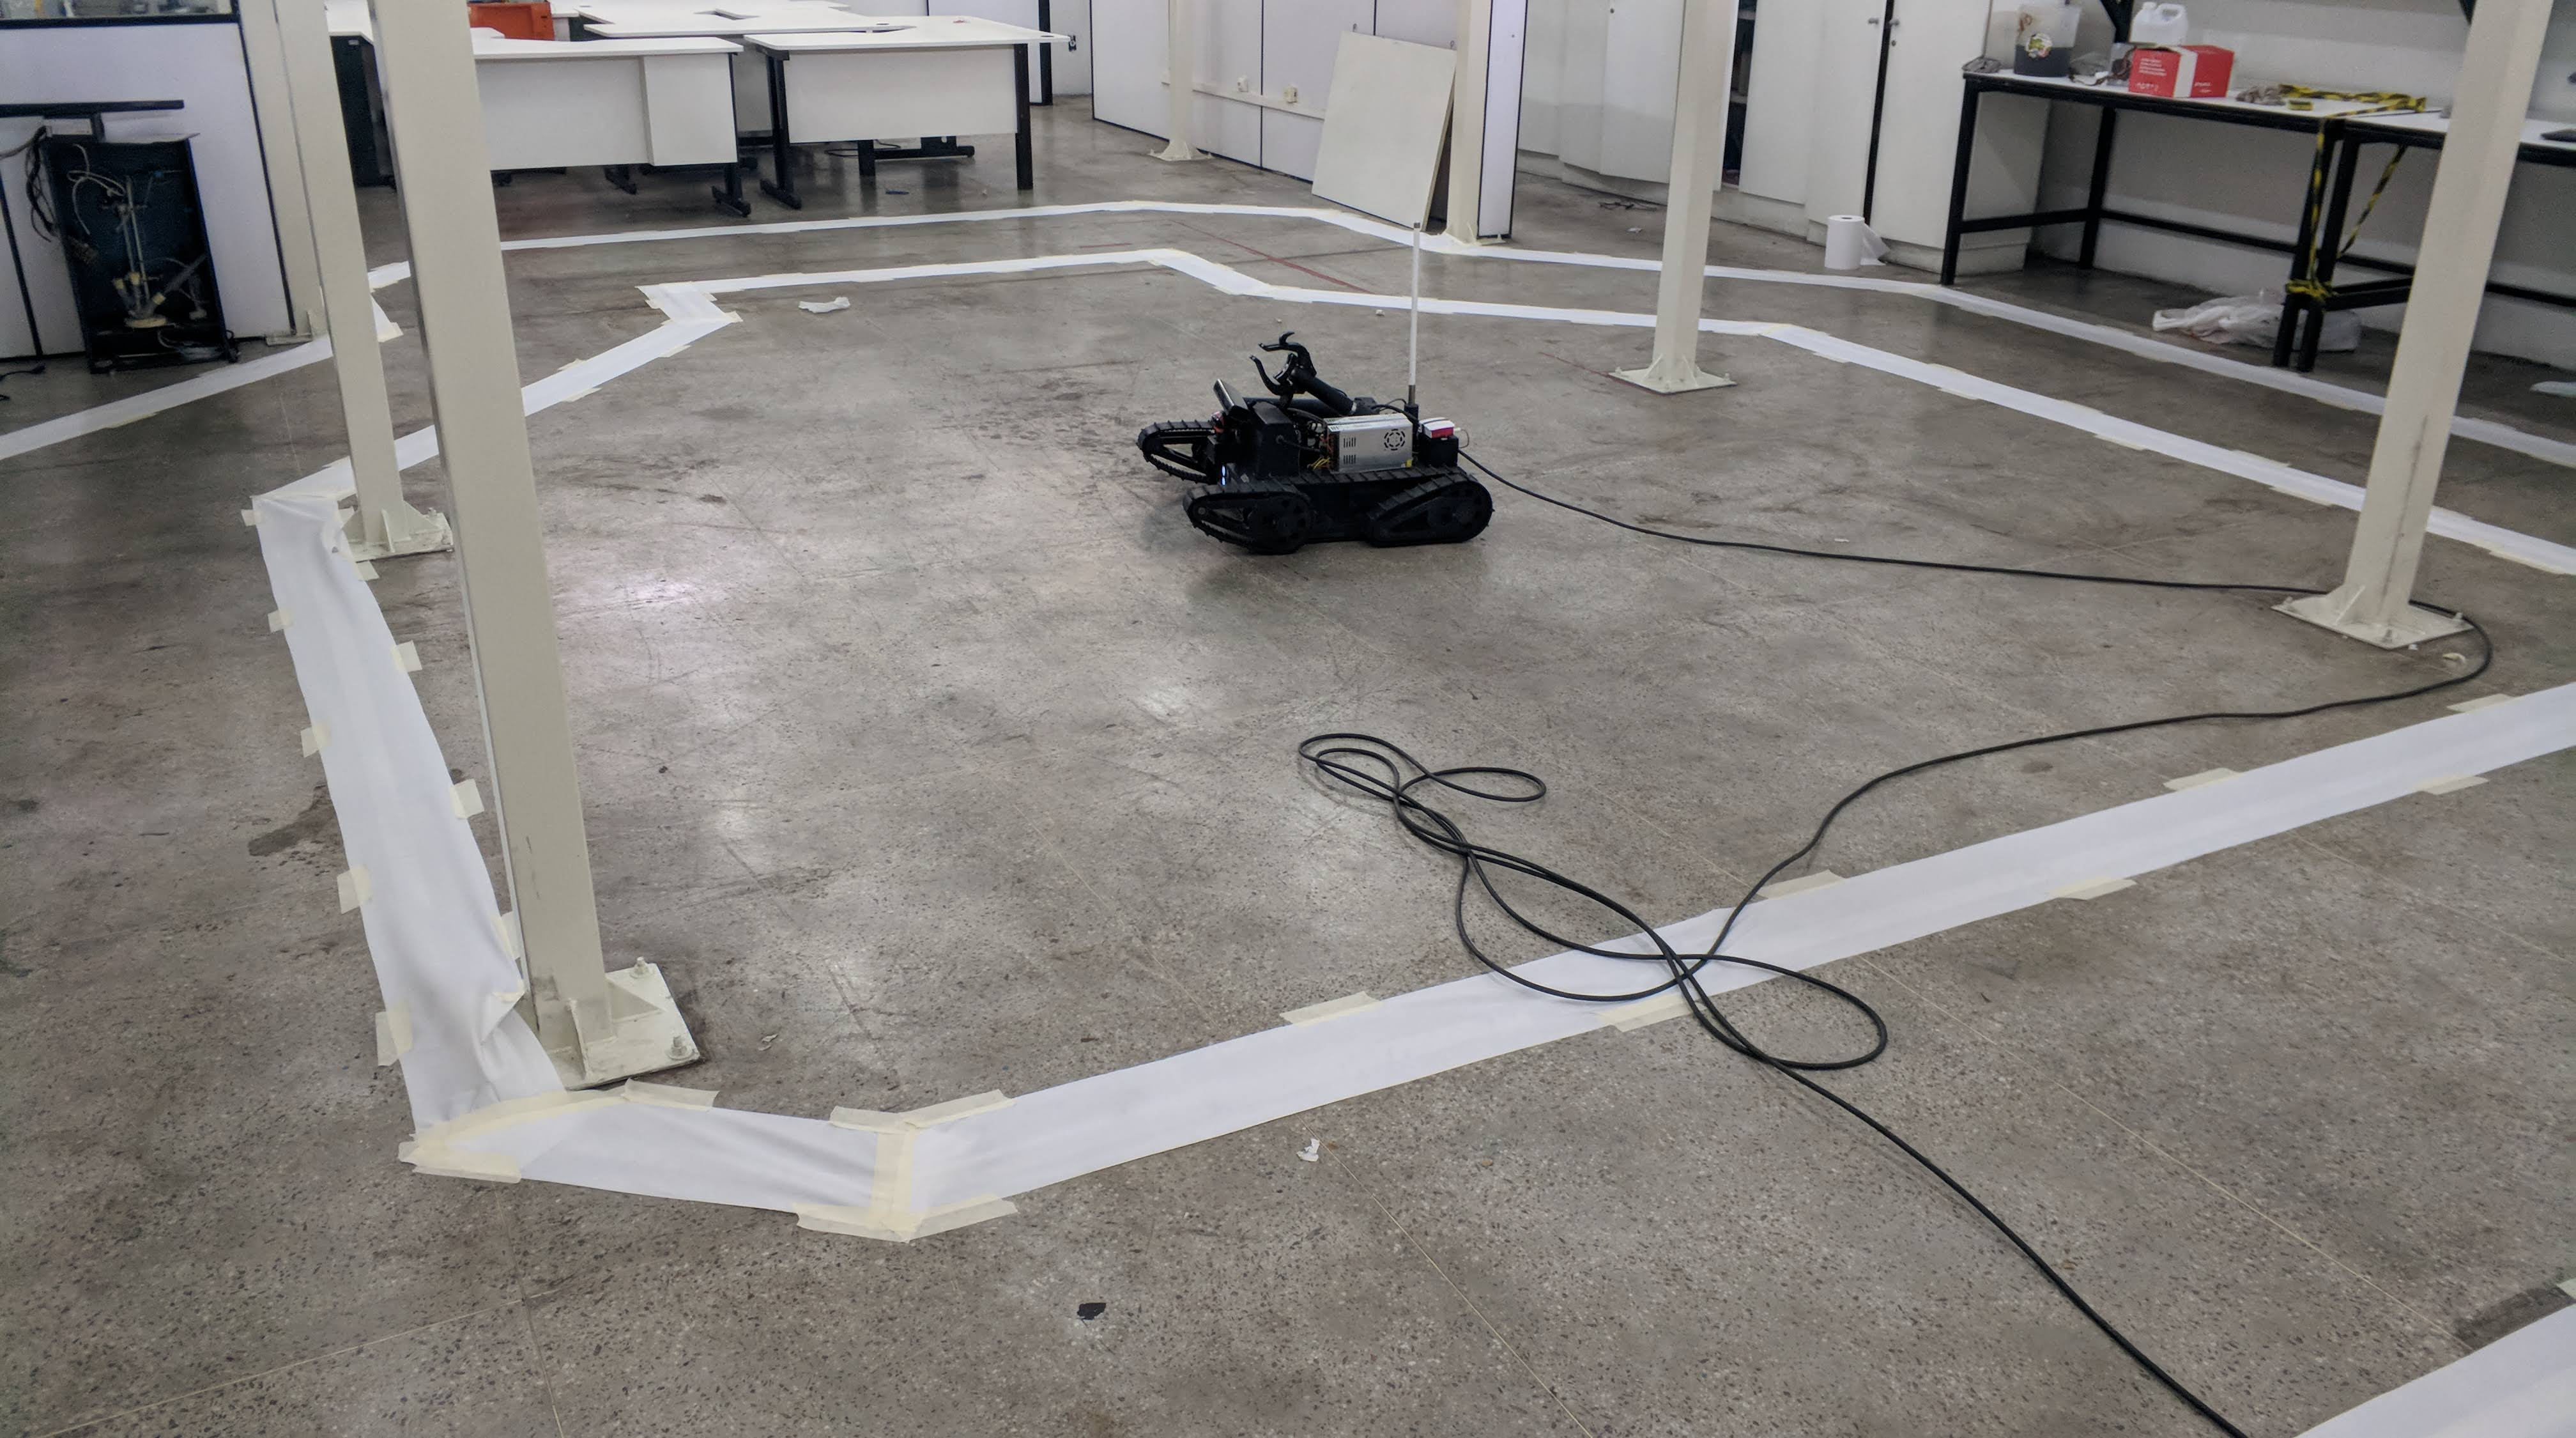
\includegraphics[width=15cm]{figuras/pis2.jpg}}
		}{
			\Fonte{Elaborado pelo autor}
		}	
\end{figure}


O grande problema da segunda pista foi o papel toalha. Toda vez que Jaguar errava alguma movimento e passava por cima da pista ele rasgava o papel toalha. Durante os testes e treinamento ela teve que ser refeita inúmeras vezes, mas pelo menos a segunda pista foi melhor para a visualização do Jaguar. 

	\begin{figure}[H]
		\centering
		\Caption{\label{imagem2} Imagem Capturada pela câmera do Jaguar}
		\UNIFORfig{}{
			\fbox{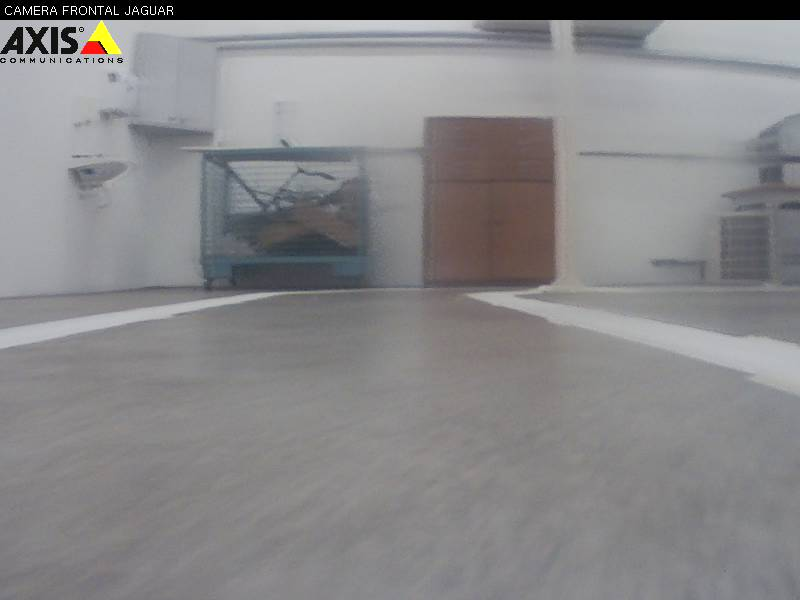
\includegraphics[width=14cm]{figuras/pista2imagemboa.jpg}}
		}{
			\Fonte{Elaborado pelo autor}
		}	
\end{figure}

A última pista foi feita do mesmo material da segunda, porém com a adição de fita zebrada amarela e preta nas bordas da pista. Como o algoritmo visualiza melhor com uma grande diferença de cores, a fita deu um destaque na pista, facilitando para o processamento. A figura \ref{pista3} mostra a aplicação da fita zebrada nas bordas da pista e a figura \ref{imagem3} mostra a mesma pista sendo visualizada pelo câmera do Jaguar.

	\begin{figure}[H]
		\centering
		\Caption{\label{pista3} Última Pista da L4}
		\UNIFORfig{}{
			\fbox{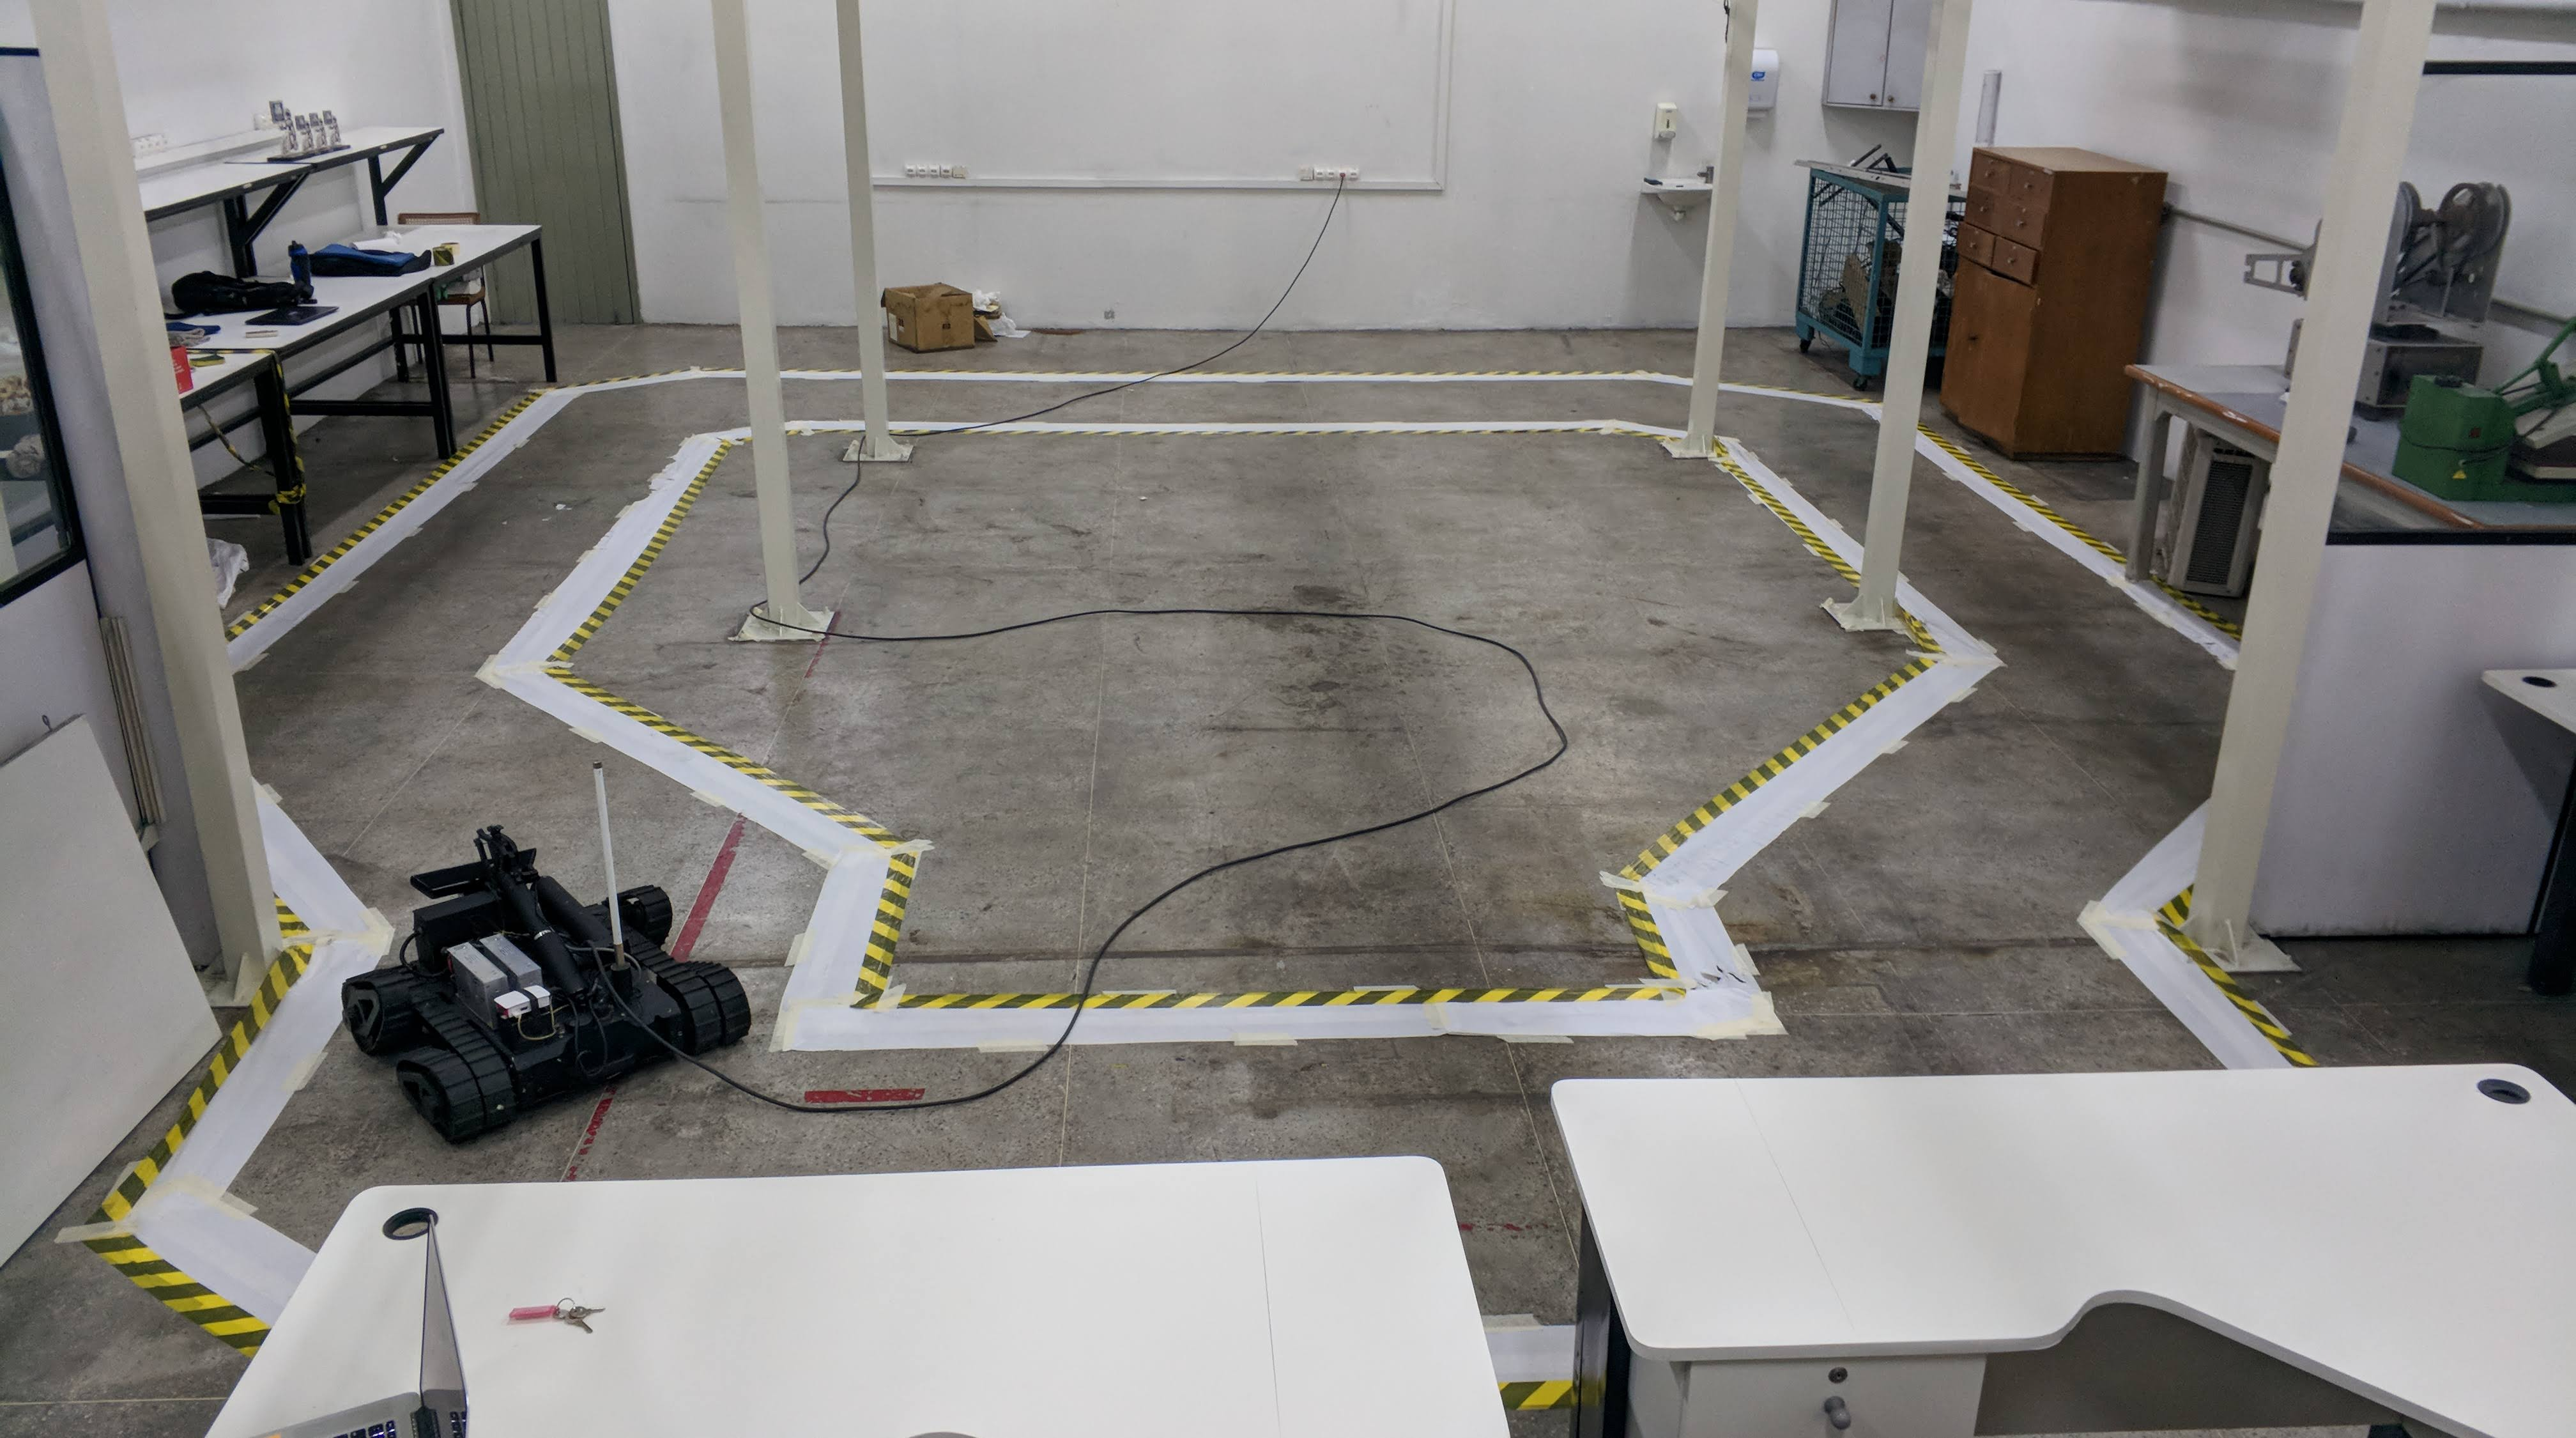
\includegraphics[width=15cm]{figuras/pista3.jpg}}
		}{
			\Fonte{Elaborado pelo autor}
		}	
\end{figure}

	\begin{figure}[H]
		\centering
		\Caption{\label{imagem3} Imagem Capturada pela câmera do Jaguar}
		\UNIFORfig{}{
			\fbox{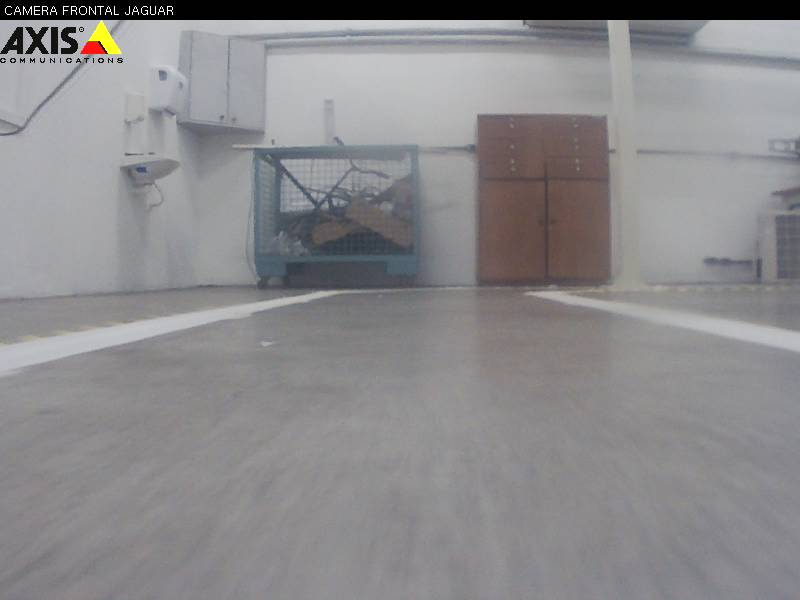
\includegraphics[width=15cm]{figuras/pista3imagemruim.jpg}}
		}{
			\Fonte{Elaborado pelo autor}
		}	
\end{figure}

Para o último caso, a rede neural foi configurada com os parâmetros da tabela \ref{tabela2}:

\begin{table}[H]
\centering
\caption{Parâmetros de treinamento do segundo modelo}
\label{tabela2}
\begin{tabular}{|l|l|l|l|}
\hline
\textbf{Treinamento} & \textbf{nb\_epoch} & \textbf{samples\_per\_epoch} & \textbf{batch\_size} \\ \hline
1º        & 20        & 2000                & 200         \\
2º        & 20        & 5000                & 150         \\
3º        & 20        & 10000               & 150         \\
4º        & 30        & 20000               & 150         \\ \hline
\end{tabular}
\end{table}

Como o número de \textit{epoch} chega ao máximo de 30, poderá haver 30 modelos diferentes, mas não foi isso o que aconteceu. Como o programa está configurado para criar um modelo somente se ele tiver o \textit{val\_loss} menor que o anterior, nem sempre haverá a mesma quantidade de modelos para a quantidade de \textit{epoch} configurada. O programa fez um treinamento para cada \textit{epoch}, mas não gerou um modelo para cada um. A tabela \ref{tabela3} mostra o resultado dos cinco melhores modelos de cada treinamento realizado da Tabela \ref{tabela2}. Nela, é possível ver o número do treinamento que saiu o modelo (Coluna treinamento), a época do modelo ou número do modelo (coluna Epoch), o tempo que levou para gerar o modelo em segundos (Coluna Tempo de Prcs.(s)), o valor do \textit{Loss} (coluna \textit{Loss}) e o valor do \textit{Val\_loss} (Coluna \textit{Val\_loss}) que é o valor mais importante pois com ele é possível saber o quanto o modelo errou na sua simulação de treinamento. Quanto menor esse valor melhor poderá ser o modelo, mas isso só pode ser testado na prática. A tabela \ref{tabela3} está organizada do menor valor de \textit{Val\_loss} (no caso, o melhor modelo) para o maior. Nos testes, os modelos 8 e 15 da tabela \ref{tabela3} tiveram os melhores resultados, como é possível ver no vídeo.



\begin{table}[H]
\centering
\caption{Melhores resultados de cada treinamento Pista 2}
\label{tabela3}
\begin{tabular}{|l|l|l|l|l|l|}
\hline
\textbf{Modelo} & \textbf{Treinamento} & \textbf{Epoch} & \textbf{Tempo de Prcs.(s)} & \textit{\textbf{Loss}} & \textit{\textbf{Val\_loss}} \\ \hline
1                   & 2º                   & 11             & 114                        & 0,0716                 & 0,031                       \\
2                   & 3º                   & 4              & 209                        & 0,0697                 & 0,033                       \\
3                   & 2º                   & 6              & 108                        & 0,0725                 & 0,035                       \\
4                   & 1º                   & 17             & 46                         & 0,0735                 & 0,0355                      \\
5                   & 2º                   & 16             & 112                        & 0,0758                 & 0,0355                      \\
6                   & 3º                   & 11             & 216                        & 0,0795                 & 0,0357                      \\
7                   & 2º                   & 10             & 129                        & 0,0687                 & 0,0358                      \\
8                   & 1º                   & 13             & 47                         & 0,0723                 & 0,0368                      \\
9                   & 2º                   & 12             & 114                        & 0,0693                 & 0,0371                      \\
10                   & 3º                   & 5              & 212                        & 0,0707                 & 0,0371                      \\
11                   & 1º                   & 12             & 46                         & 0,0734                 & 0,0385                      \\
12                   & 4º                   & 3              & 416                        & 0,0686                 & 0,0389                      \\
13                   & 1º                   & 19             & 46                         & 0,0725                 & 0,039                       \\
14                   & 3º                   & 3              & 211                        & 0,0686                 & 0,0392                      \\
15                   & 3º                   & 1              & 236                        & 0,0786                 & 0,0396                      \\
16                   & 1º                   & 10             & 46                         & 0,0726                 & 0,0401                      \\
17                   & 4º                   & 2              & 420                        & 0,067                  & 0,045                       \\
18                   & 4º                   & 4              & 421                        & 0,0705                 & 0,0458                      \\
19                   & 4º                   & 1              & 423                        & 0,0736                 & 0,0473                      \\
20                   & 4º                   & 6              & 418                        & 0,0751                 & 0,0483 \\ \hline                    
\end{tabular}
\end{table}

Em comparação com os modelos da primeira pista na sessão \ref{primeiro_teste}, o resultado do \textit{val\_loss} da segunda pista foi bem menor, o que, em teoria, era para ser o modelo melhor. Na prática, o Jaguar teve um melhor desempenho da quadra de atletismo da Unifor. Na segunda pista, localizada na sala da L4, o Jaguar enfrentou alguns problemas devido o formato da pista, com curvas muito acentuadas; a cor da parede, que era a mesma cor da borda pista; e o chão, que é da mesma cor tanto dentro quanto fora da pista. Mesmo com a função \textit{crop()} do \textit{utils.py} ainda é fica visível uma pequena parte da parede, como é possível ver na figura \ref{parede}. Tudo isso pode ter gerado uma confusão no algoritmo que gera o modelo de predição da pista. 

	\begin{figure}[H]
		\centering
		\Caption{\label{parede} Exemplo Imagem cortada da Pista 2}
		\UNIFORfig{}{
			\fbox{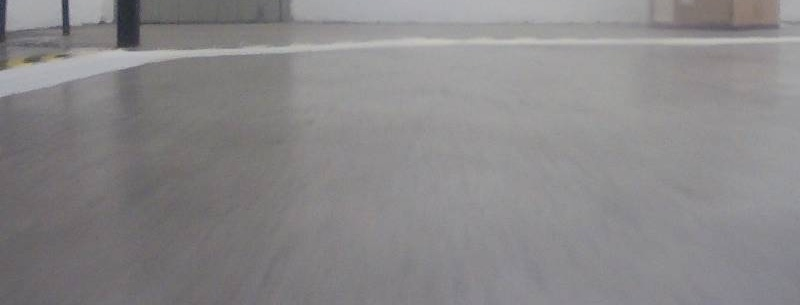
\includegraphics[width=14cm]{figuras/parede.jpg}}
		}{
			\Fonte{Elaborado pelo autor}
		}	
\end{figure}

Ao final do Projeto, O Jaguar conseguiu percorrer a pista de atletismo totalmente autônomo perfeitamente. Na segunda pista, localizada na sala da L4, ele conseguiu percorrer a pista porém em alguns momentos, principalmente próximo as paredes brancas, ele precisou de um auxílio para retornar a pista. No geral, o Jaguar conseguiu percorrer a primeira pista e boa parte da segunda, mostrando assim um resultado bem satisfatório para o projeto.
Todos os arquivos do projeto podem ser encontrados no \textit{link} do \textit{GitHub}: https://github.com/PedroUnifor/behavioral-cloning-one-camera, assim como os video no link do \textit{YouTube}:
https://youtu.be/l4X\_hcGPhMY.
	\chapter{Conclusões e Trabalhos Futuros}
\label{chap:conclusoes-e-trabalhos-futuros}

Mesmo diante de algumas limitações, o Jaguar consegue nevegar de forma autônoma. Na primeira pista o seu desempenho foi excelente, o que surpreendeu a todos pelo pouco treinamento da rede neural e escassez de recursos tanto para o teste quanto para o treinamento.

Na segunda pista o seu desempenho foi satisfatório, porém não tão bom quanto na pista de atletismo na Unifor. Em alguns momentos ele agia como se não conseguisse visualizar as bordas da pista, acabando fugindo um pouco dela. Porém, por mais que alguns momentos tivesse que parar para ajustá-lo, ele conseguiu realizar todas as curvas do percurso, satisfazendo assim as exigências básicas para a conclusão do projeto.

\section{Limitações}
\label{sec:limitacoes}

Sem dúvida a maior limitação foi a perda da bateria do Jaguar. Sem ela, foi preciso usar cabos para ligar o Jaguar diretamente na tomada, impossibilitando dele percorrer longas distâncias na quadra de atletismo na Unifor e fazer um longo percusso na sala da L4 por causa das pilastras.

Para fazer um bom treinamento é preciso ter uma grande quantidade de fotos. Algoritmos de Aprendizagem Profunda foram desenvolvidos para trabalhar com uma imensa quantidade de dados e, no caso de imagens, eles chegam a trabalhar com mais de dez mil imagens. Nesse projeto, cada treinamento foi feito com no máximo duas mil imagens devido as limitações de cabo e tempo, resultando em modelos não tão otimizados.

O material para fazer a segunda pista era o de pior qualidade. Toda vez que o Jaguar confundia uma trajetória ele destruía parte da pista e mesmo consertando ela não ficava tão perfeita quanto era antes. Isso atrapalha na hora da criação de novos modelos e até para os testes.

As cores das paredes e pistas provavelmente causaram uma confusão no algoritmo da rede neural. As bordas das pistas eram brancas, assim como as paredes da sala da L4 e o chão da pista era o mesmo chão de fora da pista. O algoritmo precisa de cores diferenciadas para saber por onde o deve percorrer. Se as cores são parecidas, provavelmente ele não vai diferenciar com clareza o que é e o que não é pista.

\section{Trabalhos Futuros}
\label{sec:trabalhos-futuros}

Esse trabalho foi apenas o pontapé inicial de um projeto que ainda pode crescer muito. Se o Jaguar for levado para outras pistas na intenção de obter novos dados de treinamento será possível aperfeiçoar ainda mais o seu modelo de navegação autônoma. Além disso, o jaguar possui sensores como GPS  (sistema de posicionamento global) e \textit{LiDAR} (sensor que mede a distância de objetos próximos) que podem ser utilizados para trabalharem juntos com a câmera e o algoritmo de inteligência artificial aperfeiçoando ainda mais a navegação autônoma da plataforma.

	%Elementos pós-textuais
	\bibliography{elementos-pos-textuais/referencias}
	\imprimirglossario
	\imprimirapendices
		% Adicione aqui os apendices do seu trabalho
		\apendice{Lorem Ipsum}
\label{ap:lorem-ipsum}

\lipsum[1]
		\apendice{Modelo de Capa}
\label{ap:modelo-de-capa}

\lipsum[1]

		\apendice{Termo de Fiel Depositário}
\label{ap:termo-de-fiel-depositario}

\noindent \textbf{Pesquisa:} ANÁLISE DA MORTALIDADE INFANTIL COM MALFORMAÇÕES CONGÊNITAS.

\noindent Pelo presente instrumento que atende às exigências legais, a Sra. Maria Consuelo Martins Saraiva, ``fiel depositário'' com o cargo de Secretária Municipal de Saúde de Iracema, após ter tomado conhecimento do protocolo de pesquisa intitulado: ANÁLISE DA MORTALIDADE INFANTIL COM MALFORMAÇÕES CONGÊNITAS. Analisando a repercussão desse estudo no contexto da saúde pública e epidemiologia, autoriza Karla Maria da Silva Lima, enfermeira, aluna do Curso de Mestrado Acadêmico em Enfermagem da Universidade Estadual do Ceará (UECE), sob orientação do Prof. Dr. José Maria de Castro, da UECE, ter acesso aos bancos de dados do Sistema de Informação sobre Nascidos Vivos e do Sistema de Informação sobre Mortalidade da Secretaria Municipal de Saúde de Iracema, objeto deste estudo, e que se encontram sob sua total responsabilidade. Fica claro que o Fiel Depositário pode a qualquer momento retirar sua AUTORIZAÇÃO e ciente de que todas as informações prestadas tornar-se-ão confidenciais e guardadas por força de sigilo profissional, assegurando que os dados obtidos da pesquisa serão somente utilizados para estudo.
	\imprimiranexos
		% Adicione aqui os anexos do seu trabalho
		\anexo{Exemplo de Anexo}
\label{an:exemplo-de-anexo}

\lipsum[13]
		\anexo{Dinâmica das classes sociais}
\label{an:dinamica-das-classes-sociais}

\lipsum[14]
\index{AAA}
	\imprimirindice

\end{document}
